\section{実験と分析}

本研究では、ミニ2048におけるNタプルネットワークの学習性能を多角的に分析するため、
構造の異なる複数のプレイヤを構築し、GreedyおよびExpectimax探索による評価を行った。

\ref{tuples}で示した15種類のプレイヤを用いて評価を行った。

さらに、Optimistic Initialization(OI)の影響を調べるため、
各プレイヤについてOIの初期値を0、1200、5400に設定し、それぞれ学習を実施した。
すべてのプレイヤは $5 \times 10^8$ 手分の行動に基づいて学習を行い、
乱数シードを変えて10体ずつ学習させた。結果として、
$15$タプル構成$\times 3$回(OIの初期値)$\times 10$回(シード)で,計$450$体のプレイヤが作成された。

これらのプレイヤに対して、GreedyプレイおよびExpectimax探索(深さ2〜5)による1000ゲームプレイを行い、
そのログを用いて解析を行なった。

図\ref{fig:score_vs_tuple_greedy}および\ref{fig:score_vs_tuple_exp5}には、GreedyプレイとExpectimax探索(深さ5)におけるタプル数の変化によるスコアの変化を示す。
TNは各タプルにおして平均値の高かったものを選択している。

図\ref{fig:score_vs_tuple_greedy}を見ると、GreedyプレイにおいてはNT5までのタプル数でスコアが向上していることがわかる。
NT5~NT7までOI=1200だけ横ばい、それ以外は下落している、NT8以降はすべてスコアが低下している。
これは図\ref{fig:score_vs_tuple_exp5}のExpectimax深さ5も同様の傾向が見られ、図では示していないが、
Expectimax深さ2~4についても同様の傾向が見られた。
またNT6以降のスコアはGreedy、Expectimax深さ2~5のいずれもOI=1200のスコアが高くなっている。
これはOI=1200の初期値が効果的に作用した結果であると考えられる。

ではそれぞれのタプルについて、
OIの値が変わることでどのようなスコアの変化があったか、
またそれらを用いてExpectimax探索を行った場合にどのようなスコアの変化があったかを
について詳しく見ていく。

NT1とNT2についてはOIの値が変わってもスコアの変化はほぼ見られなかった。
Expectimax探索の深さを深くした場合については、スコアは探索の深さに比例して上昇している。
図\ref{fig:exp_trendsNT3}を見るとNT3はTN=2673の方がいずれのOIでもTN144と比べてスコアが高くなってる。
探索の深さを深くした場合については、同様にスコアは探索の深さに比例して上昇しているが上下関係は変わらない。
図\ref{fig:exp_trendsNT4}を見るとNT4はTN=44755、OI=0のスコアが最も低く、それに続いてTN=301の各OIの値が続き、TN=44755の値が続いている。
探索の深さを深くした場合スコアの順序が入れ替わっている。
図\ref{fig:exp_trendsNT5}を見るとNT5はTN=896673が高く、TN=298が低い傾向にあり、
Expectimax探索の深さを深くした場合で少しスコアの差が縮まっている。
図\ref{fig:exp_trendsNT6}を見るとNT6はOIごとのスコアがちかく、TN間の差がほぼない、これはTN=16で盤面の情報を保存するのに十分なパラメータ数が
あるからだと考えられる。探索の深さを深くした場合の変化は小さいがスコアの向上が見られた。
図\ref{fig:exp_trendsNT7}、図\ref{fig:exp_trendsNT8}を見るとNT7、NT8についてはこれまでの傾向と異なりTN=0の方がスコアが高くなっている。
これにより、パラメータ数を増やして一つの盤面から得られる情報を増やしても
得点の向上につながらないことが分かる。
またNT8とNT9はNT7と比べて明確にスコアが低下している、
これは盤面の汎化性能が低下することが原因だと考えられる。
NT9についてはOI=1200のスコアが高くなっている。

全体の傾向としてOIの値が探索に与える影響は感じられなかったが、
OI=1200のスコアが高くなっていることからOIの初期値が高すぎず低すぎない適切な値に設定することが
スコアの向上に寄与していることが分かる。
またタプルサイズを増やすことやタプルの数を増やすことは、一定程度までは得点に寄与するが、
あるラインを超えると逆にスコアが低下することが分かる。
% 図は順番に挿入
% \begin{figure}[htbp]
%     \centering
%     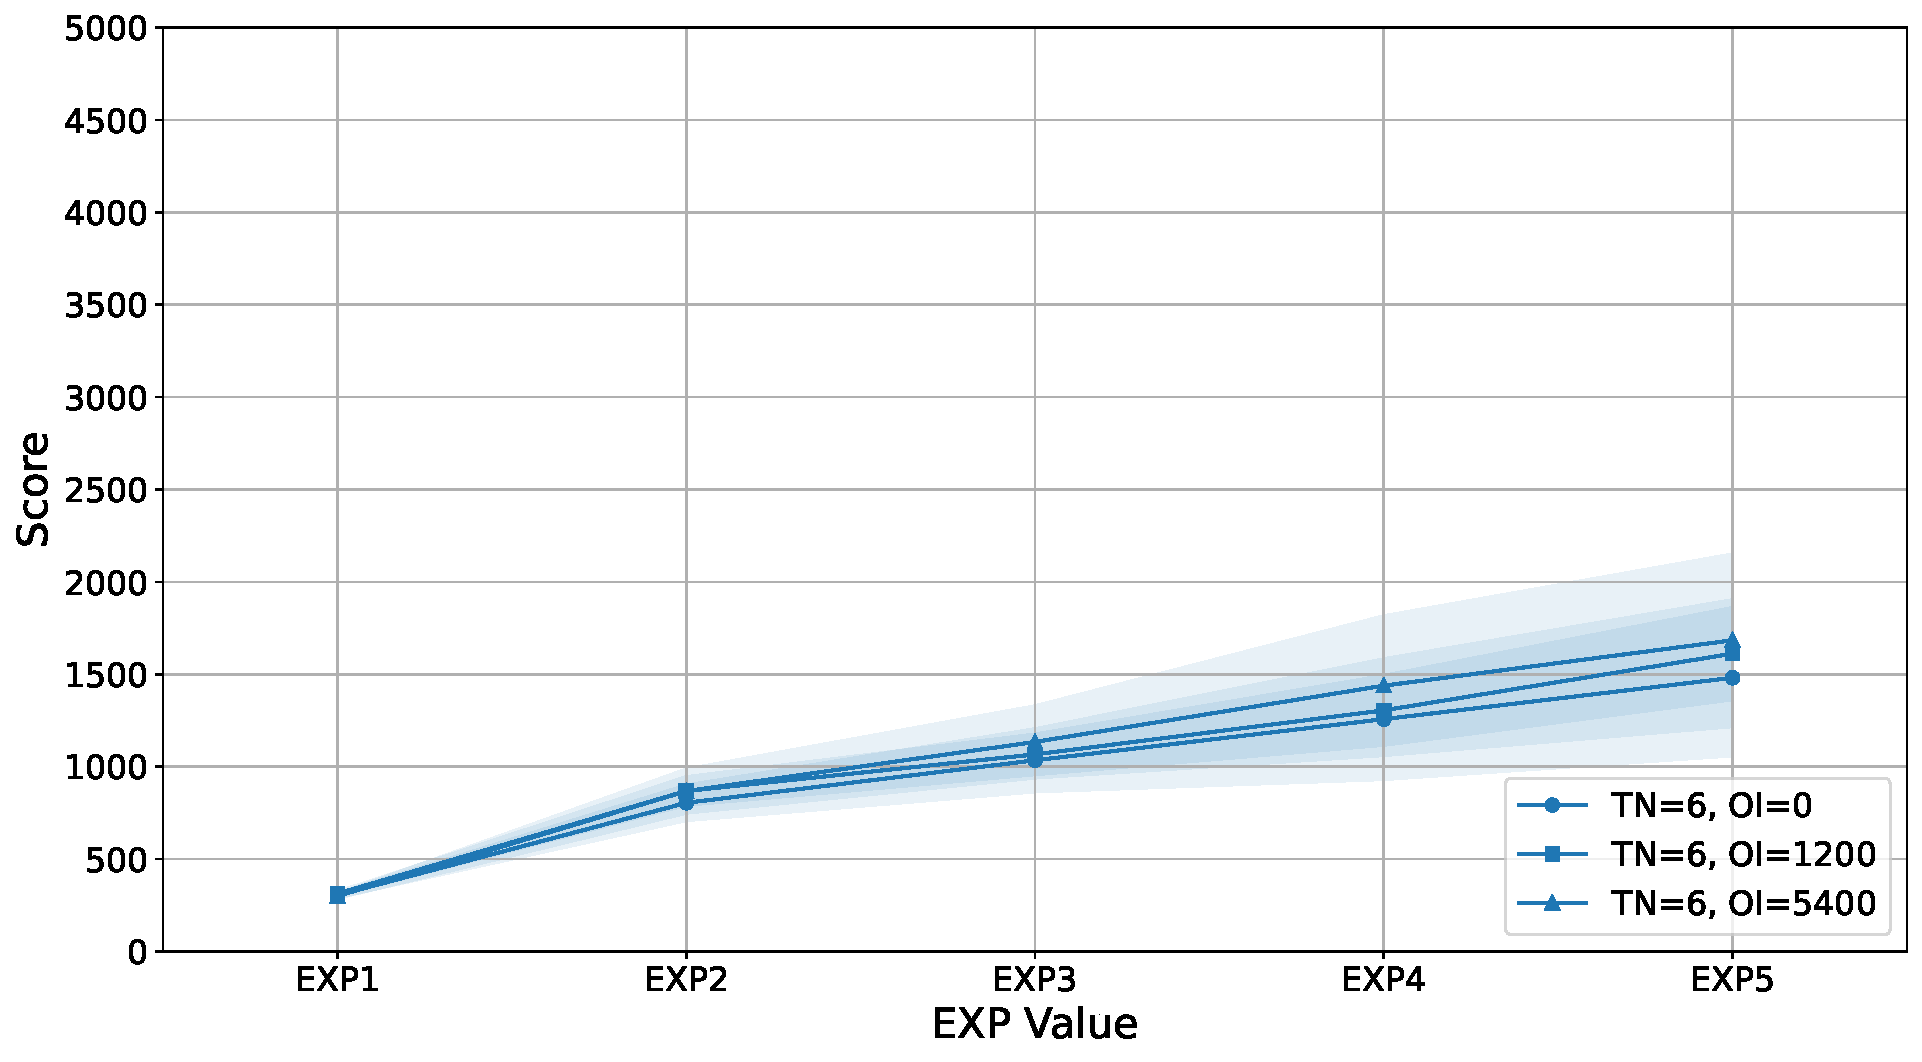
\includegraphics[width=\linewidth]{pdf/exp_trends/combined_trends_NT1.pdf}
%     \caption{実験結果の傾向NT1}
%     \label{fig:exp_trendsNT1}
% \end{figure}
% \begin{figure}[htbp]
%     \centering
%     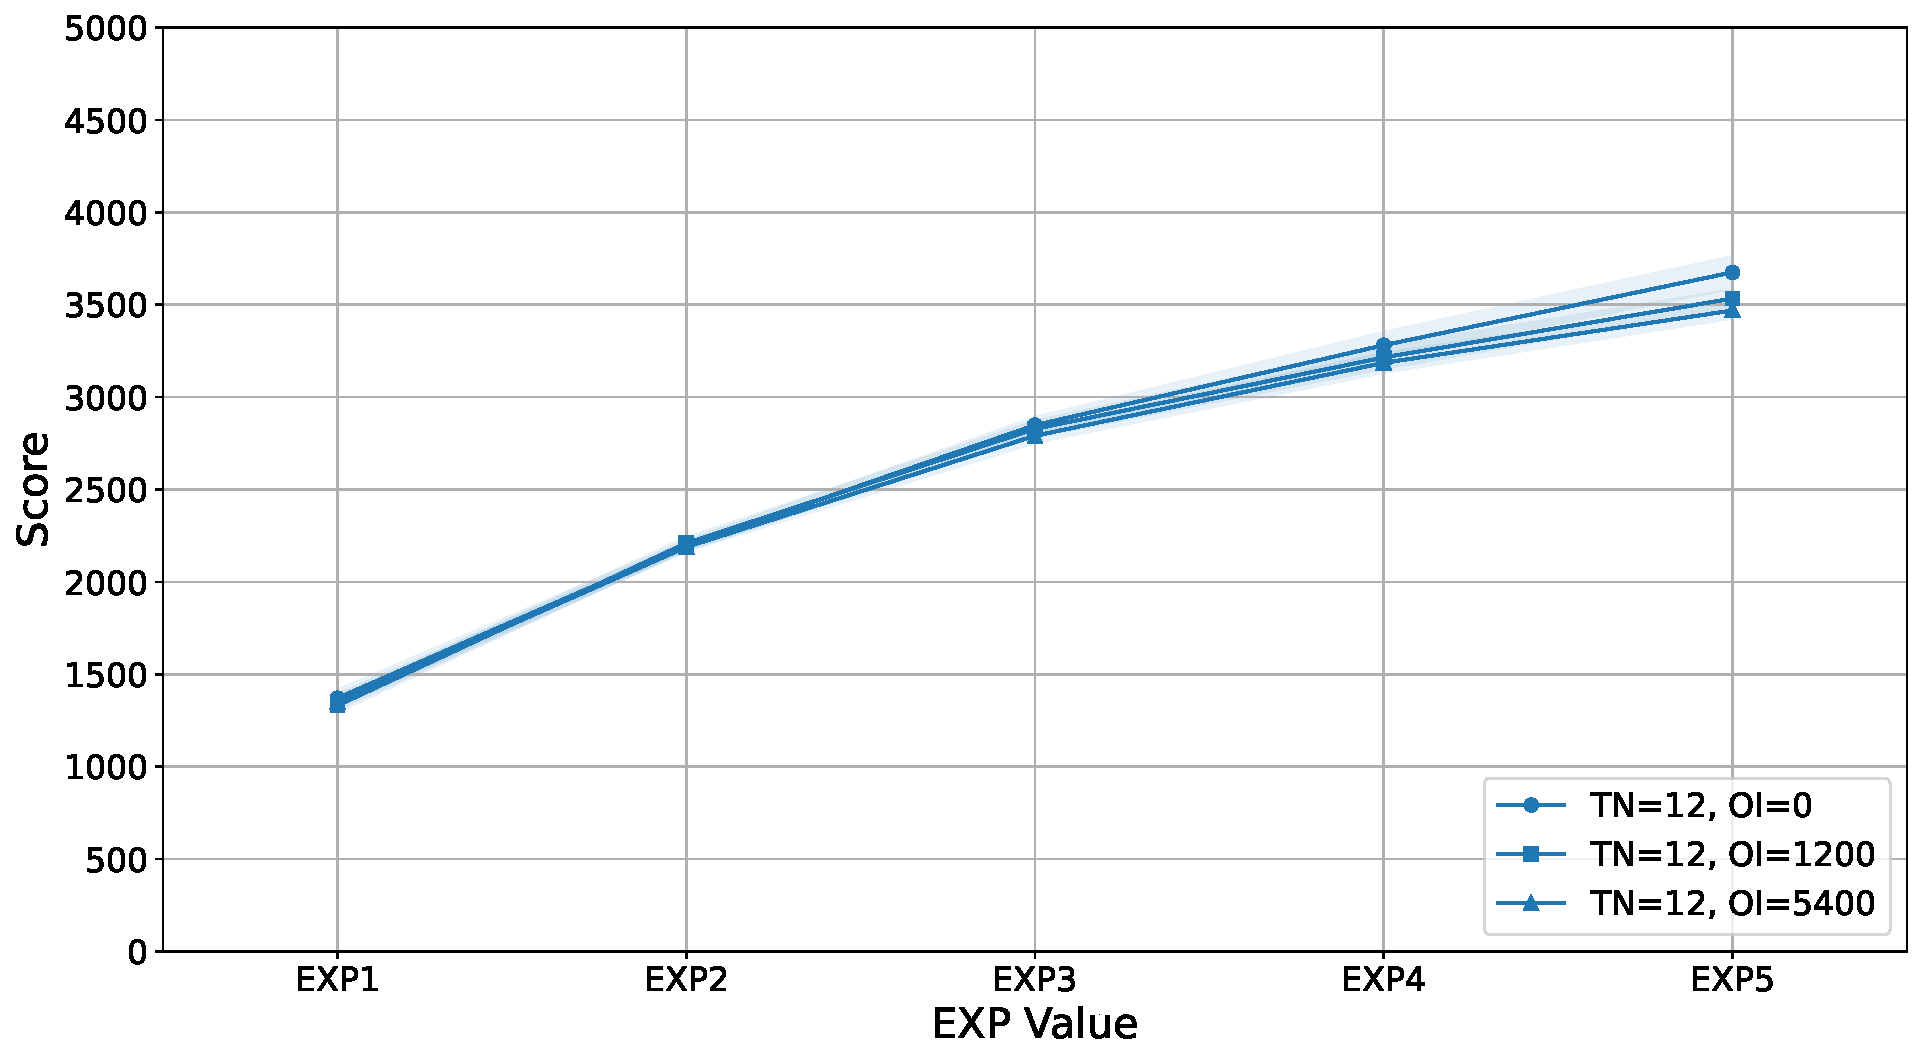
\includegraphics[width=\linewidth]{pdf/exp_trends/combined_trends_NT2.pdf}
%     \caption{実験結果の傾向NT2}
%     \label{fig:exp_trendsNT2}
% \end{figure}
\begin{figure}[t]
    \centering
    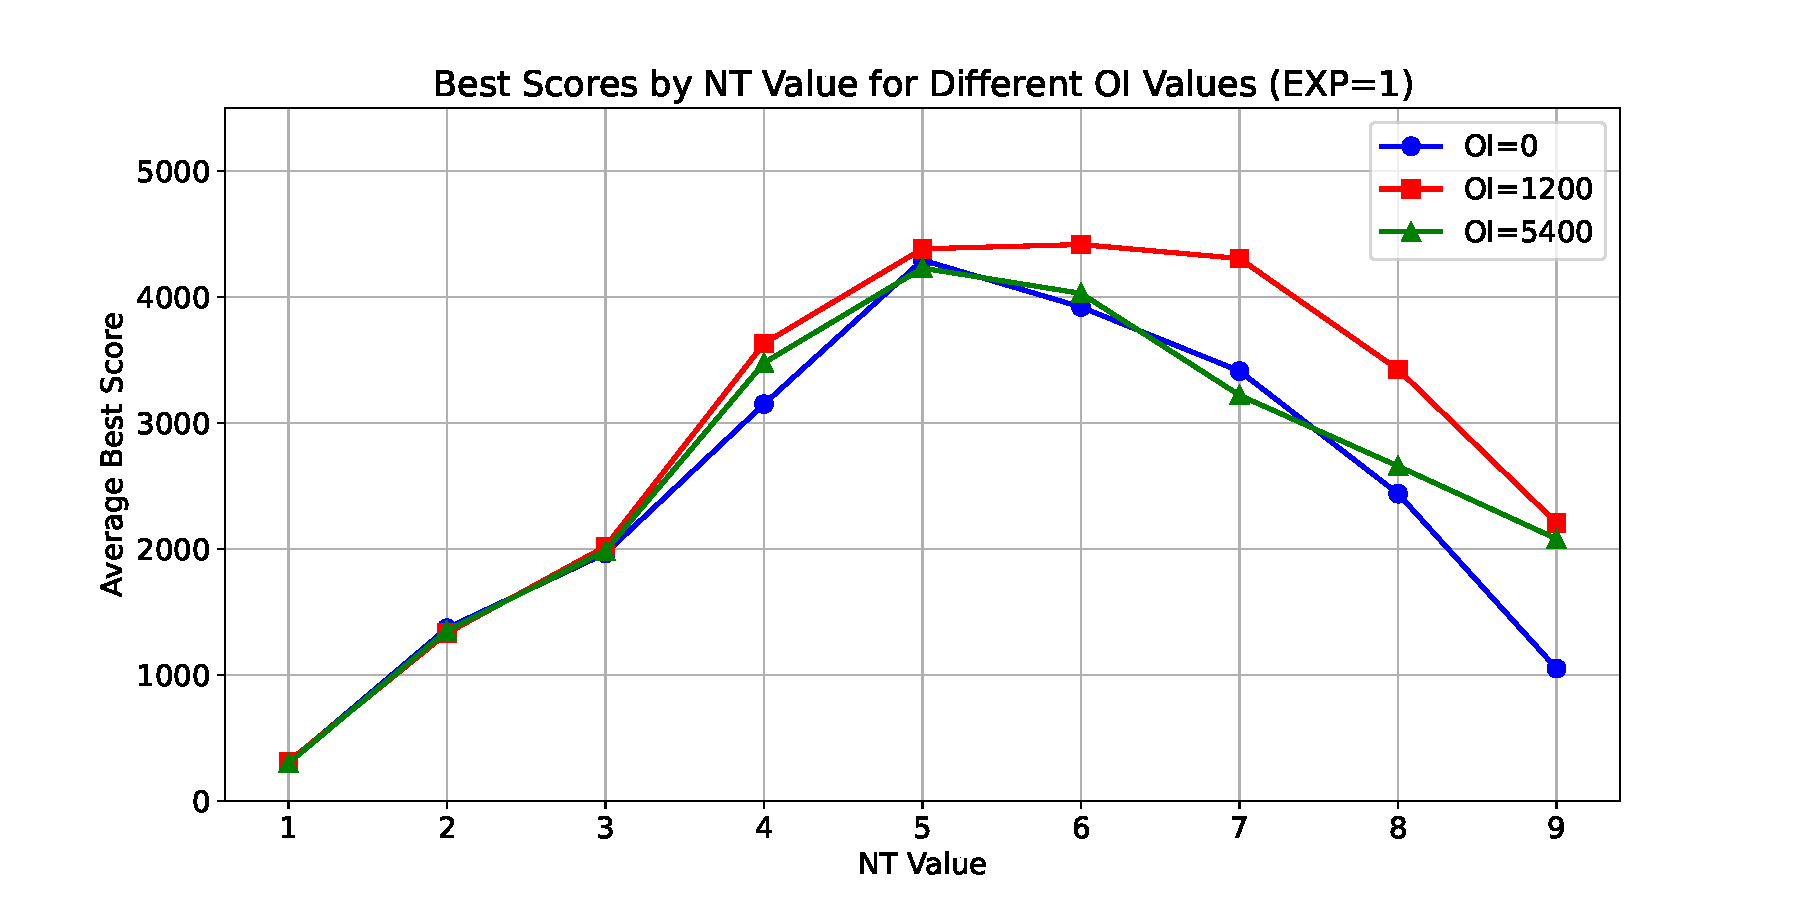
\includegraphics[width=\linewidth]{pdf/best_tn_scores_exp1.pdf}
    \caption{タプル数の変化によるスコアの変化(Greedy プレイ)}
    \label{fig:score_vs_tuple_greedy}
\end{figure}

\begin{figure}[t]
    \centering
    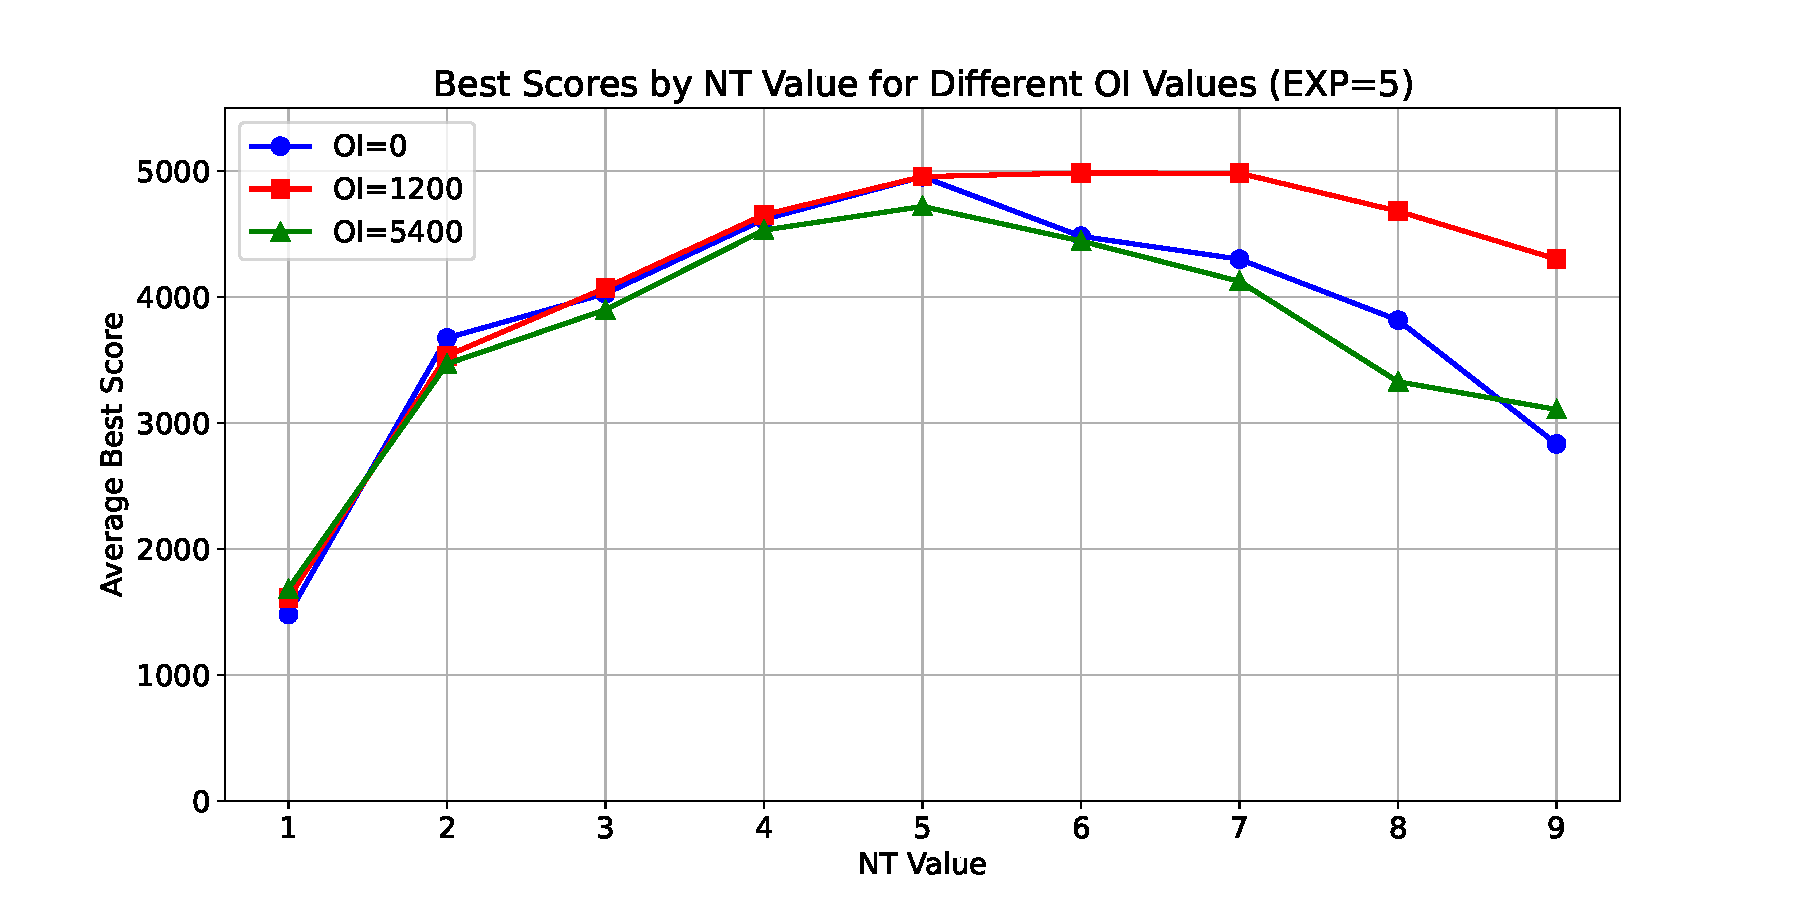
\includegraphics[width=\linewidth]{pdf/best_tn_scores_exp5.pdf}
    \caption{タプル数の変化によるスコアの変化(Expectimax 深さ5)}
    \label{fig:score_vs_tuple_exp5}
\end{figure}

\begin{figure}[t]
    \centering
    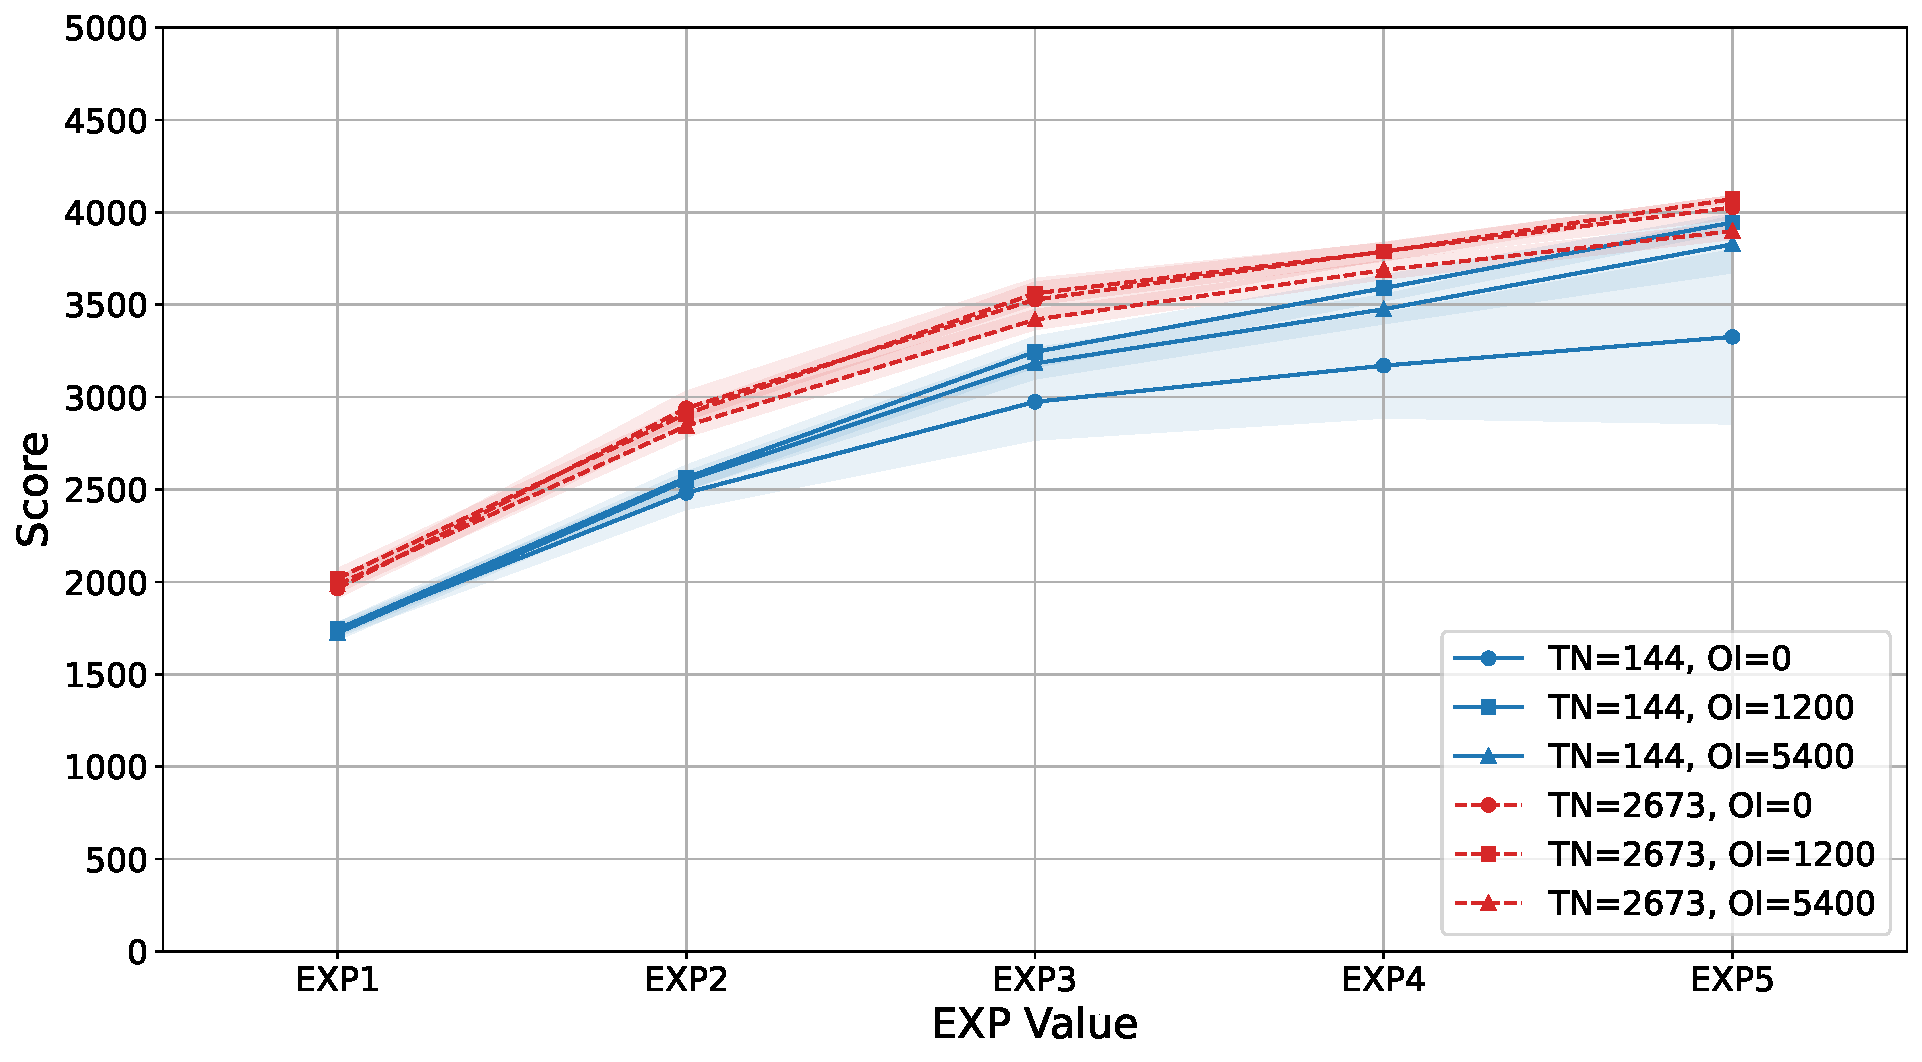
\includegraphics[width=\linewidth]{pdf/exp_trends/combined_trends_NT3.pdf}
    \caption{実験結果の傾向NT3}
    \label{fig:exp_trendsNT3}
\end{figure}
\begin{figure}[t]
    \centering
    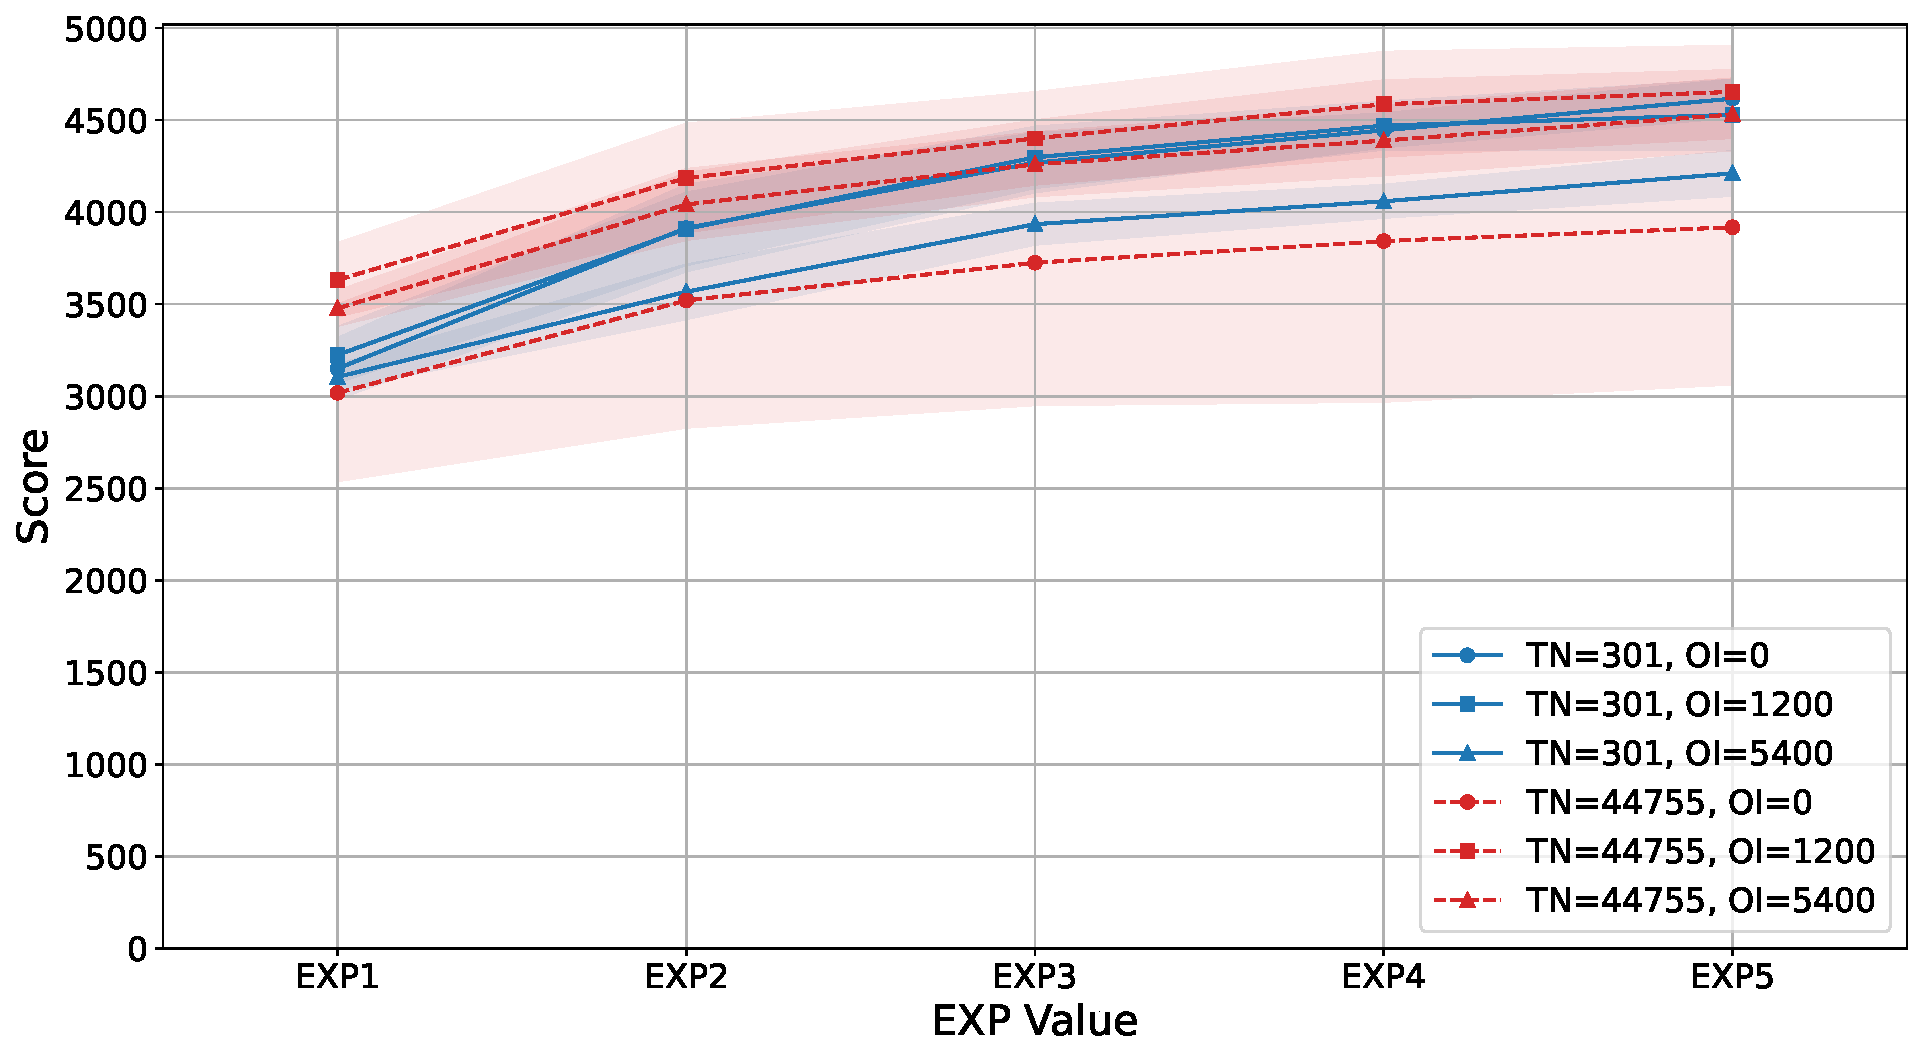
\includegraphics[width=\linewidth]{pdf/exp_trends/combined_trends_NT4.pdf}
    \caption{実験結果の傾向NT4}
    \label{fig:exp_trendsNT4}
\end{figure}
\begin{figure}[t]
    \centering
    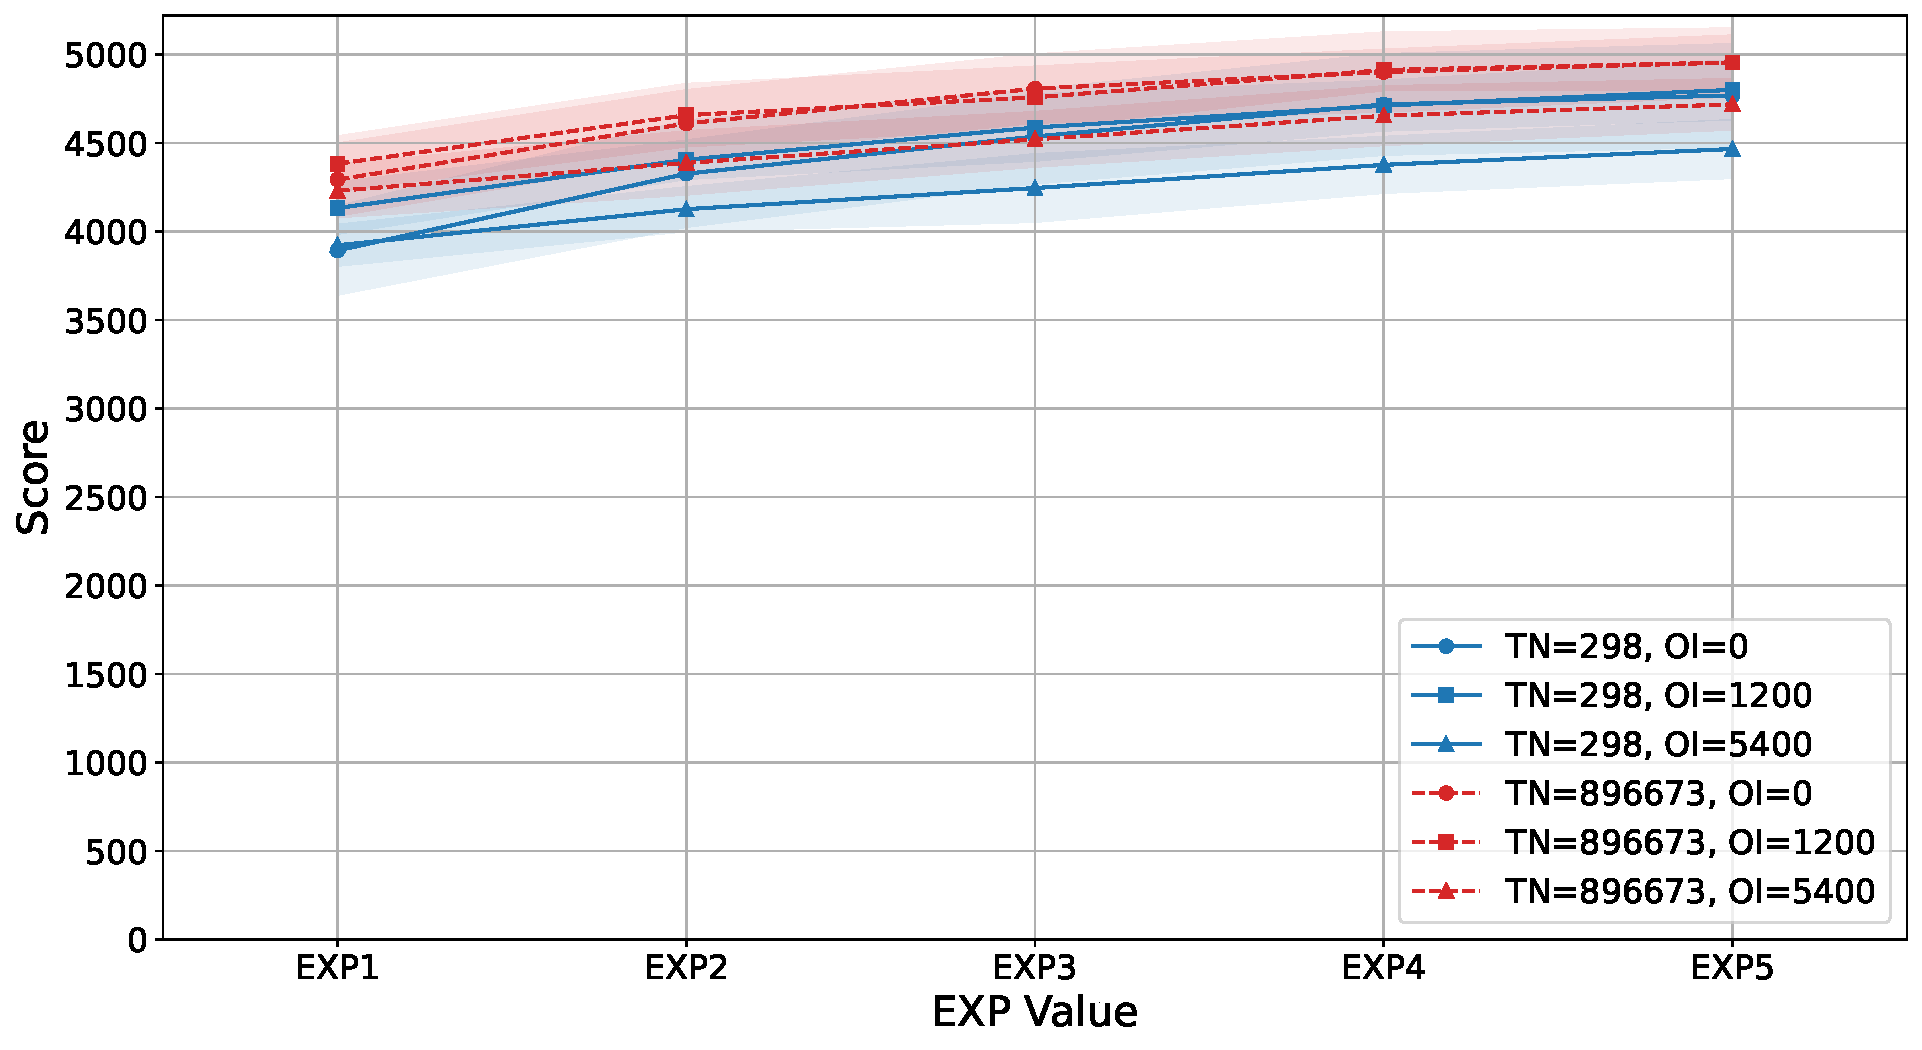
\includegraphics[width=\linewidth]{pdf/exp_trends/combined_trends_NT5.pdf}
    \caption{実験結果の傾向NT5}
    \label{fig:exp_trendsNT5}
\end{figure}
\begin{figure}[t]
    \centering
    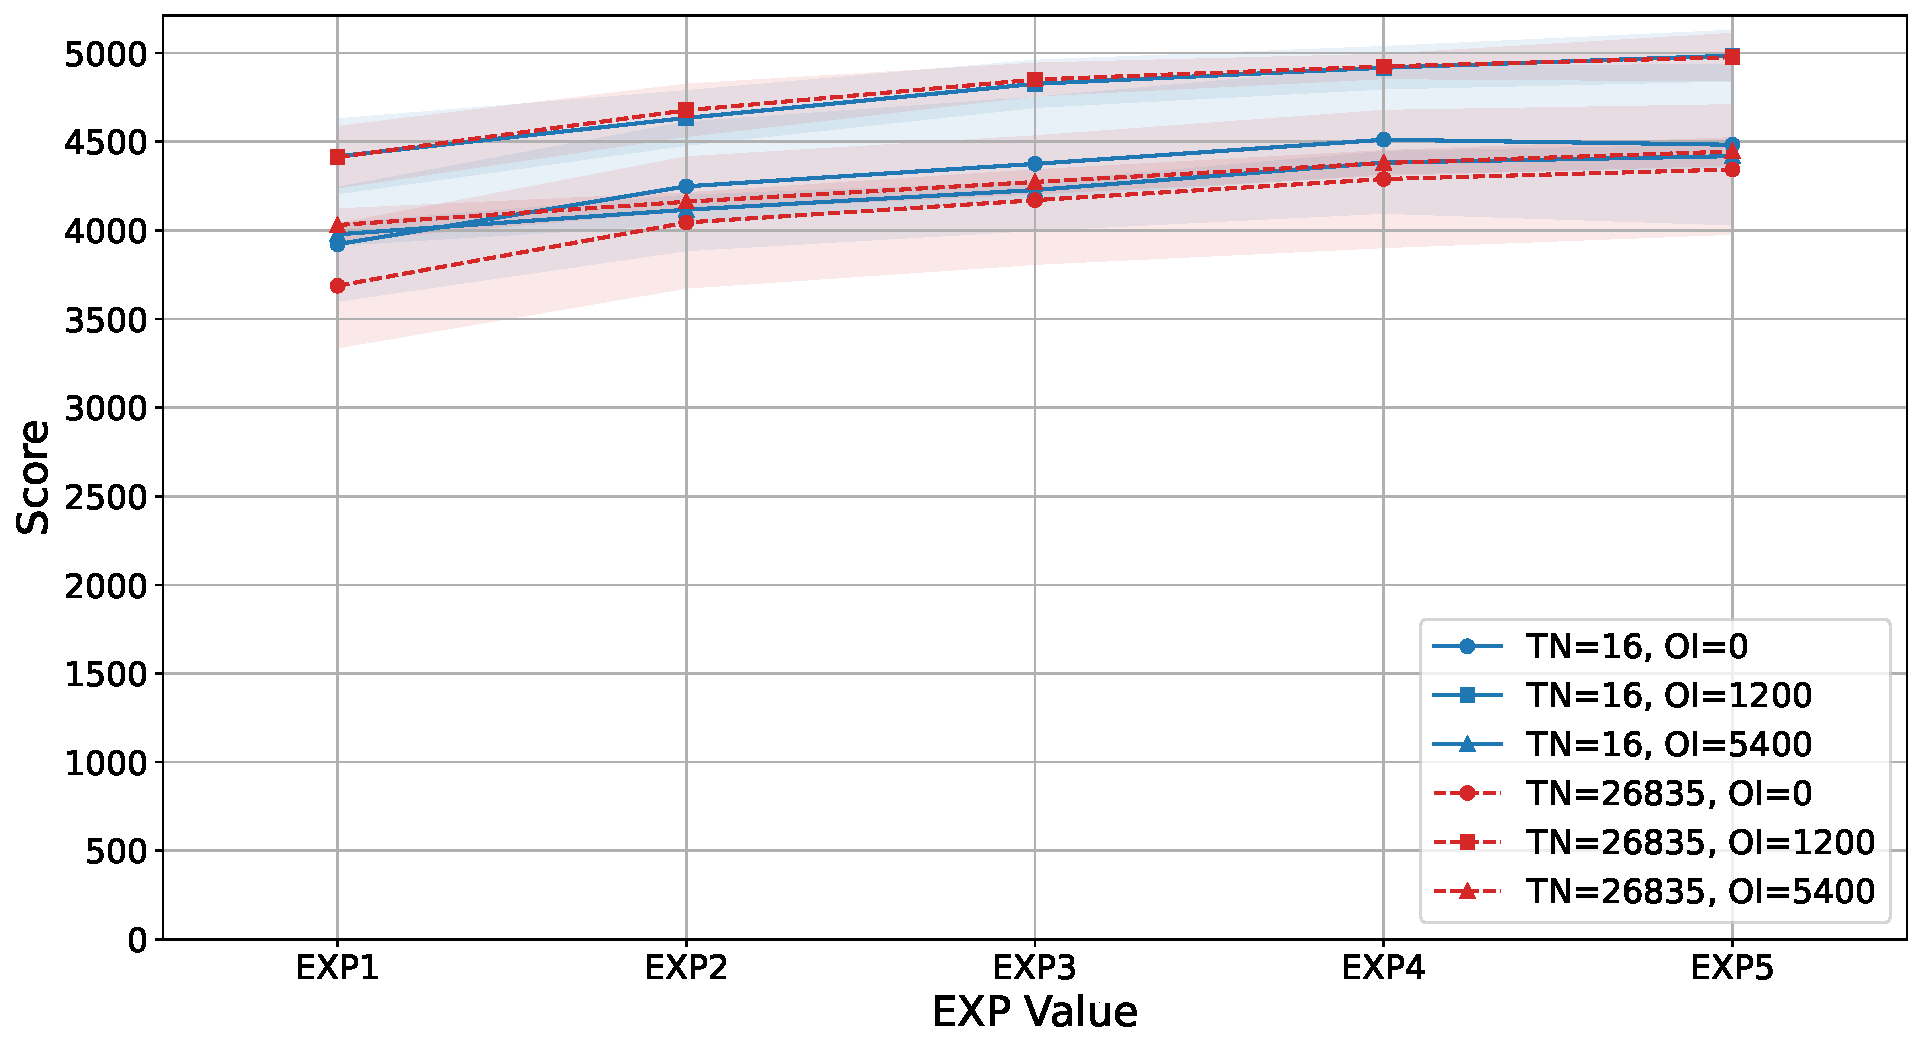
\includegraphics[width=\linewidth]{pdf/exp_trends/combined_trends_NT6.pdf}
    \caption{実験結果の傾向NT6}
    \label{fig:exp_trendsNT6}
\end{figure}
\begin{figure}[t]
    \centering
    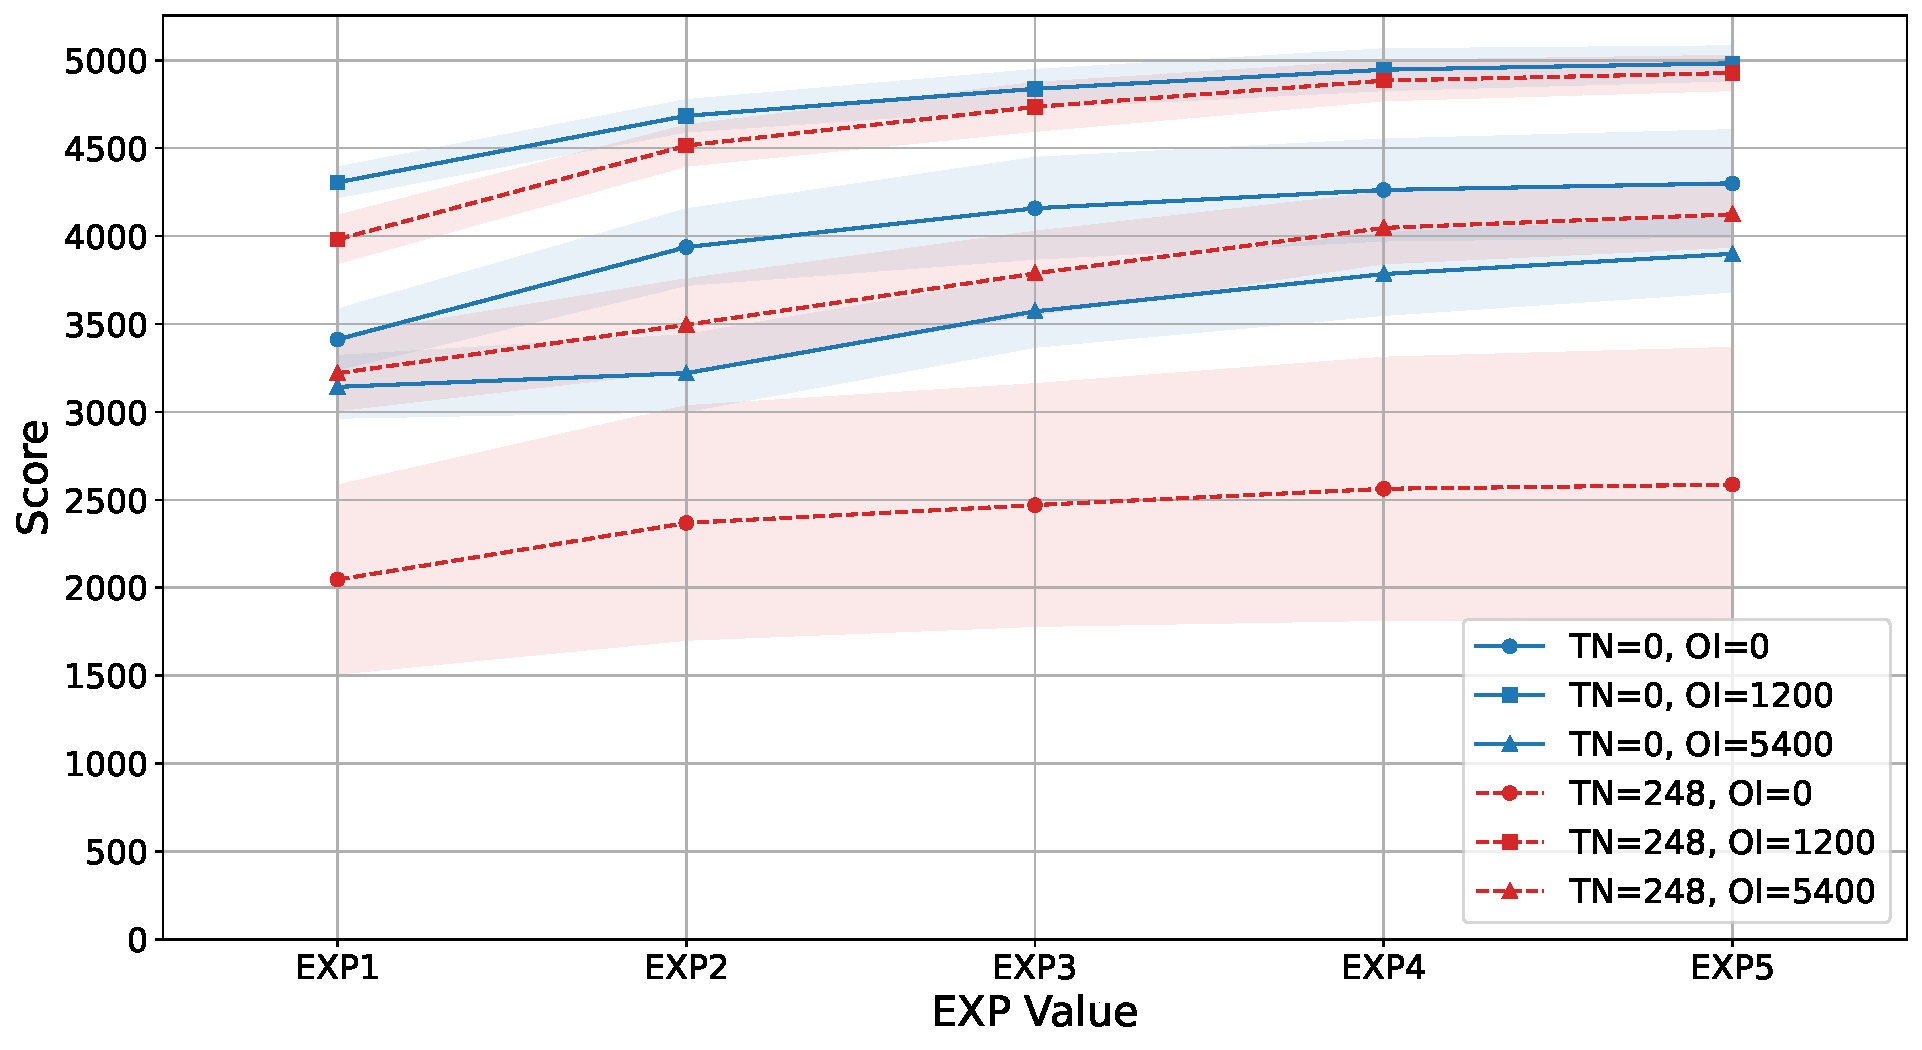
\includegraphics[width=\linewidth]{pdf/exp_trends/combined_trends_NT7.pdf}
    \caption{実験結果の傾向NT7}
    \label{fig:exp_trendsNT7}
\end{figure}
\begin{figure}[t]
    \centering
    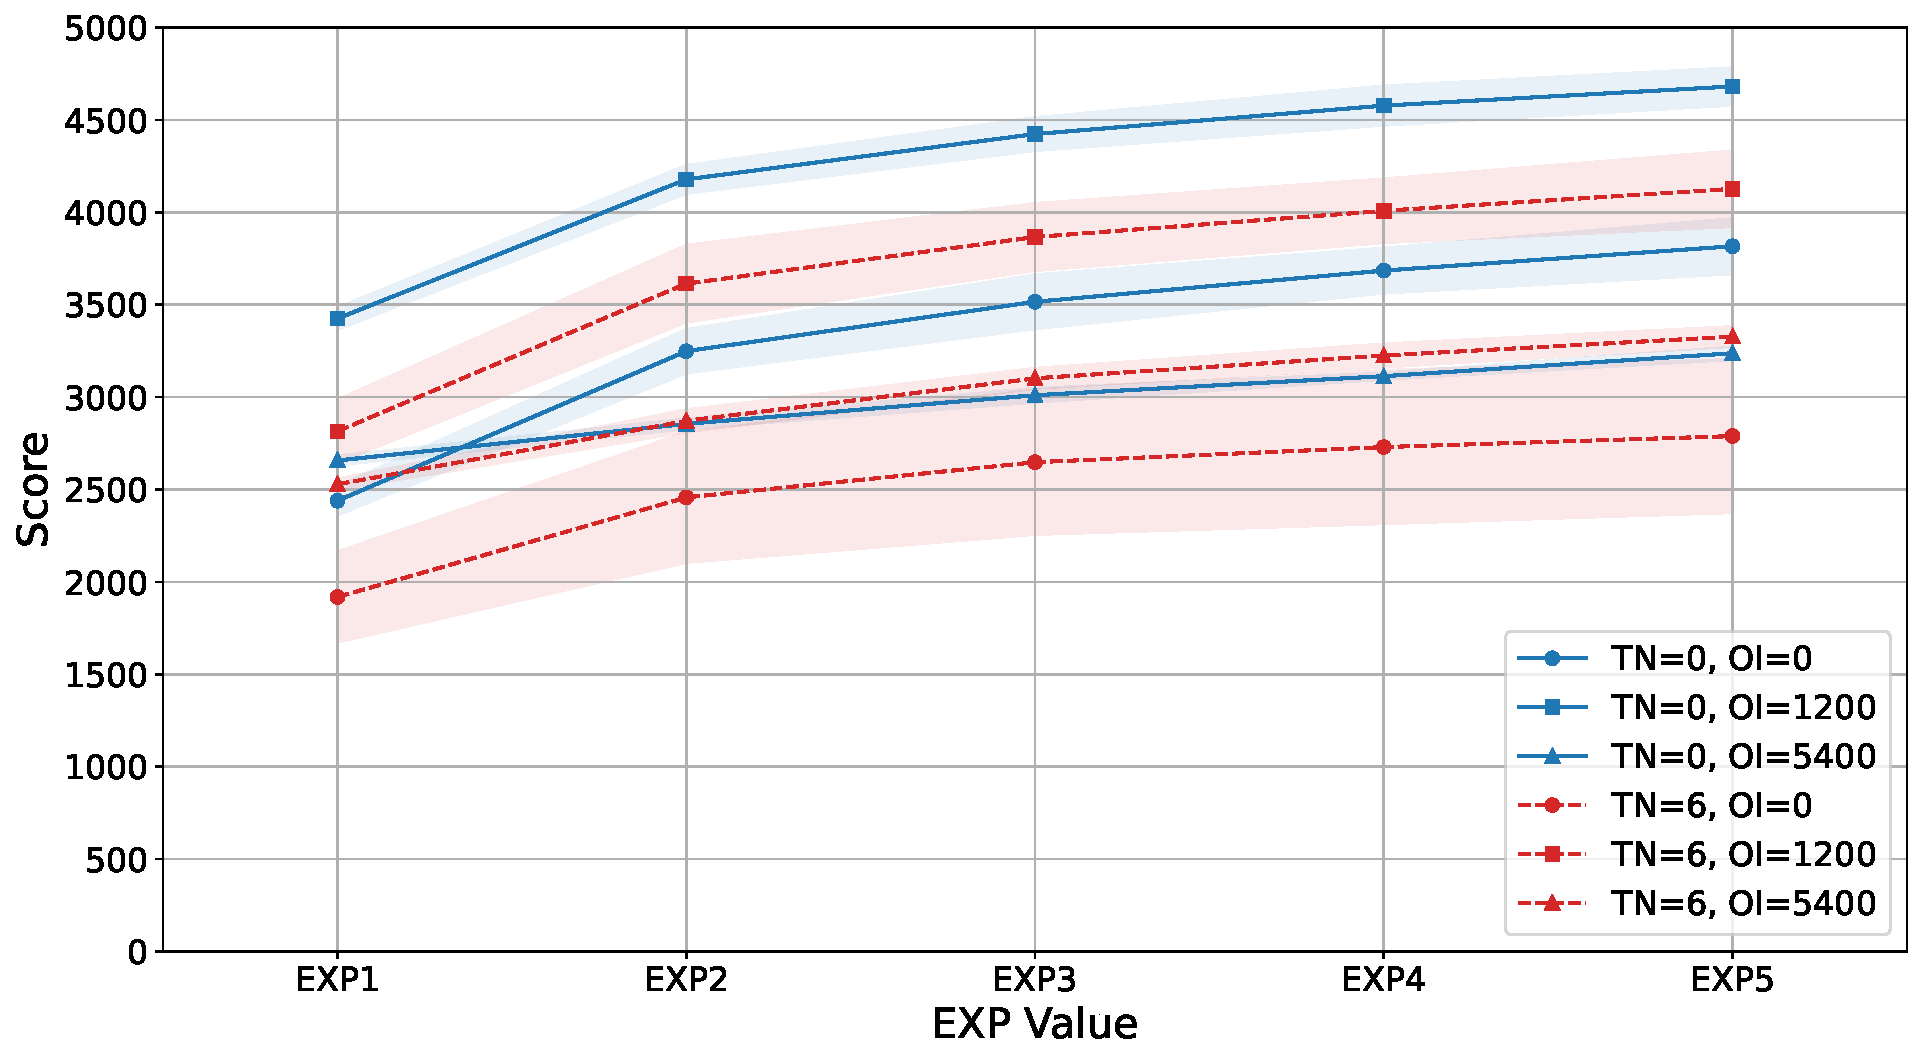
\includegraphics[width=\linewidth]{pdf/exp_trends/combined_trends_NT8.pdf}
    \caption{実験結果の傾向NT8}
    \label{fig:exp_trendsNT8}
\end{figure}
% \begin{figure}[htbp]
%     \centering
%     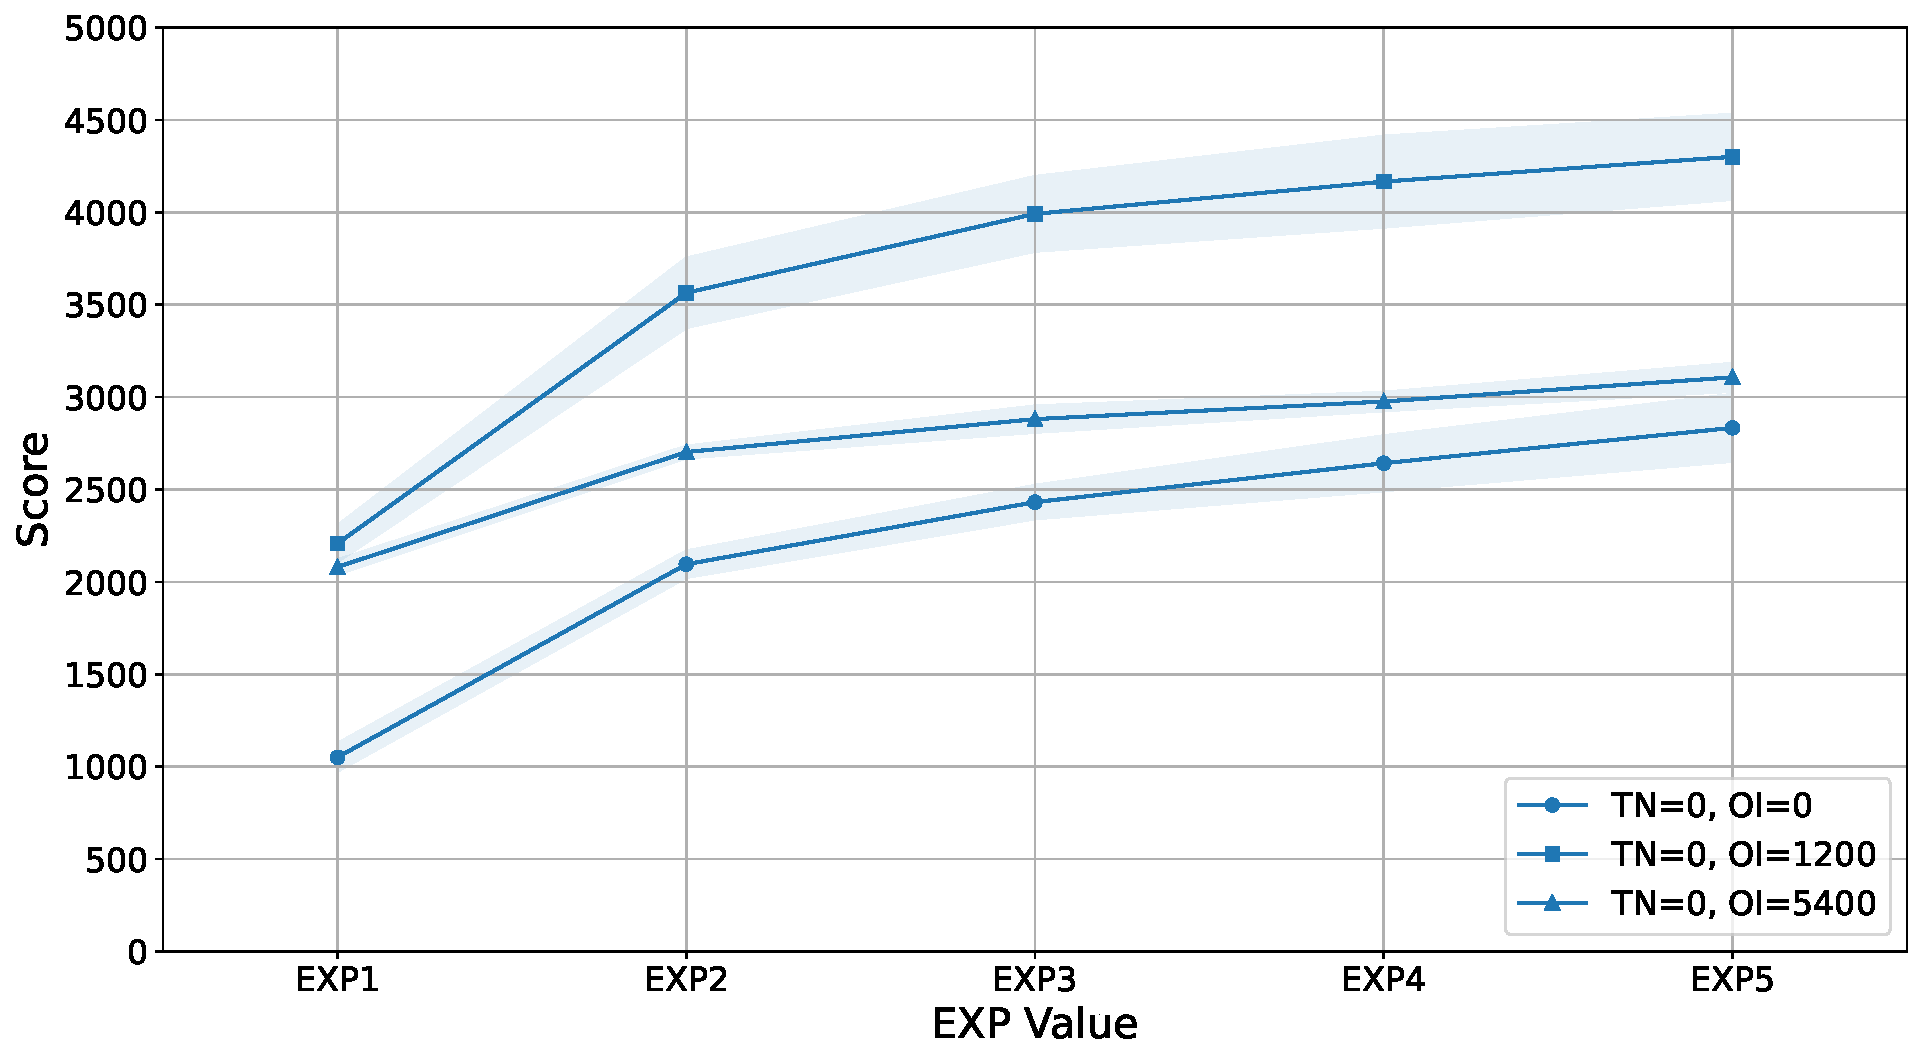
\includegraphics[width=\linewidth]{pdf/exp_trends/combined_trends_NT9.pdf}
%     \caption{実験結果の傾向NT9}
%     \label{fig:exp_trendsNT9}
% \end{figure}

NT5のTNの違いによってどのように変化するのかを見ていく、
図\ref{fig:nt5_exp1_results}はOI=1200のGreedyプレイの場合は、
TN=896673の方がスコアが高くなっている。
正確度はTN896673の方が少し高くなっているが、絶対誤差はほぼ差がない。
生存率を見るとprogress=250辺りの難易度の高い領域で生まれた生存率の差が、
正確度の差分を見ると、0.2ポイントほどprogress300辺りで差があるが、
progress250辺りの難易度の高い領域では正確度の差分があまりないことがわかる。
平均得点に200点ほどの差があるが、これは絶対誤差を見るにprogress=250辺りの少し
差がある所の積み重ねがこの差になっていると考えられる。

NT8のTNの違いによってどのように変化するのかを見ていく、
図\ref{fig:nt8_exp1_results}はOI=1200のGreedyプレイの場合は、
TN=0の方がスコアが高くなっている。
正確度と正確度の差分を見ると、
序盤のprogress100~130,170~200辺りにTN6の方が正確度が高いが、
そこの絶対誤差を見るとTN0の値がほぼ高い。
これを見ると、TN0は間違った選択をしても評価値はあまり変わらず。
TN6の場合は間違った選択をすると評価値が大きく変わることが読み取れる。

NT5のEXP5のTNの違いによってどのように変化するのかを見ていく、
図\ref{fig:nt5_exp5_results}はOI=1200のGreedyプレイの場合は、
TN=896673の方がスコアが高くなっている。
正確度はTN896673の方が高くなっているprogressが多いが、
絶対誤差はほぼ差がない。
生存率を見るとprogress=250辺りの難易度の高い領域少し差が生まれているが、
平均得点の差が生まれる要因がどこにあるのか分からない。

NT8のEXP5のTNの違いによってどのように変化するのかを見ていく、
図\ref{fig:nt8_exp5_results}はOI=1200のGreedyプレイの場合は、
TN=0の方がスコアが高くなっている。
正確度はTN0の方が高くなっているprogressが多いが、
絶対誤差はほぼ差がない。
正確度の差分を見ると波のような形で序盤の正確度が上下に揺れているが、
その間に生存率の差が生まれている。
絶対誤差のグラフを見ると、TN0の方が序盤少し高い場面が多いことが分かる。

\begin{figure}[t]
\centering
\begin{subfigure}[b]{0.49\linewidth}
    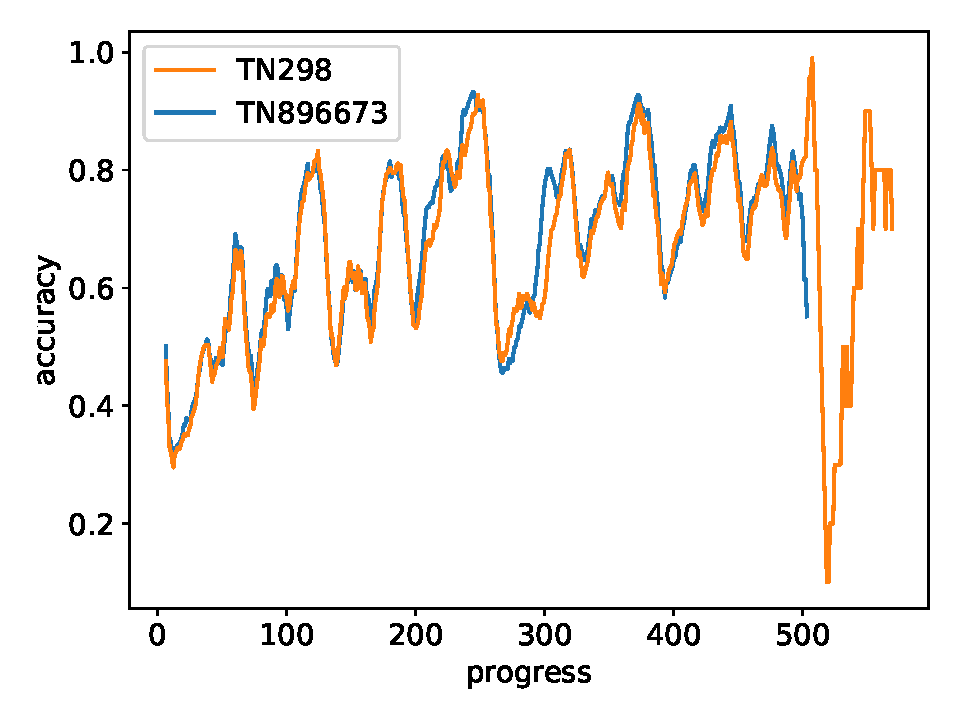
\includegraphics[width=\linewidth]{pdf/compare/merged_NT5_OI1200_compare/accuracy.pdf}
    \caption{正確度}
    \label{fig:nt5_exp1_accuracy}
\end{subfigure}
\begin{subfigure}[b]{0.49\linewidth}
    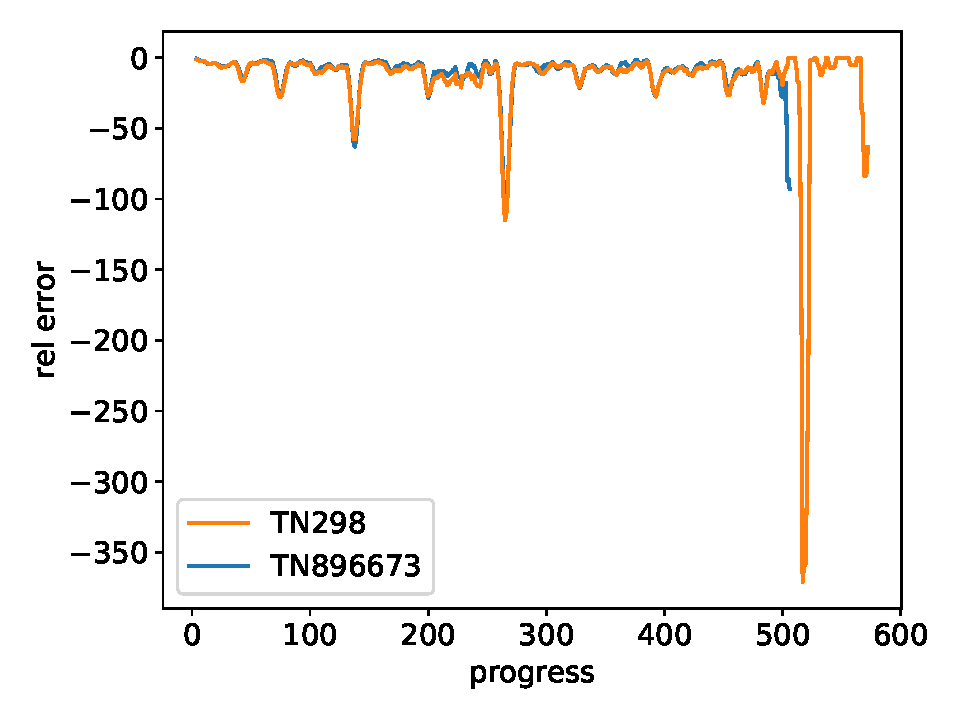
\includegraphics[width=\linewidth]{pdf/compare/merged_NT5_OI1200_compare/error_abs.pdf}
    \caption{絶対誤差}
    \label{fig:nt5_exp1_error_abs}
\end{subfigure}
% \begin{subfigure}[b]{0.49\linewidth}
%     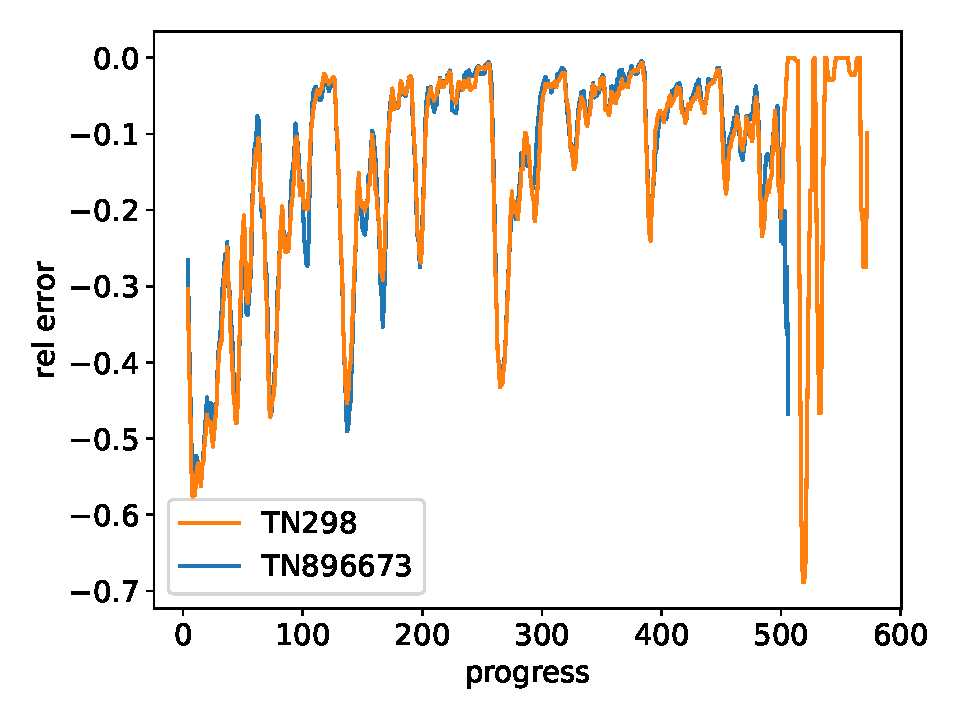
\includegraphics[width=\linewidth]{pdf/compare/merged_NT5_OI1200_compare/error_rel.pdf}
%     \caption{相対誤差}
%     \label{fig:nt5_exp1_error_rel}
% \end{subfigure}
\begin{subfigure}[b]{0.49\linewidth}
    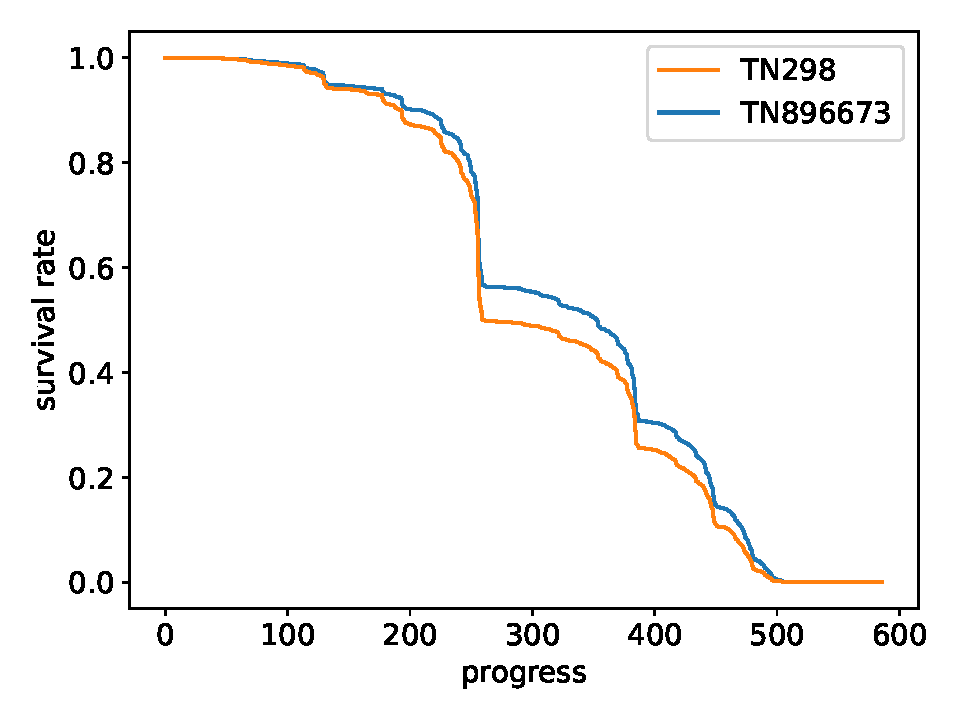
\includegraphics[width=\linewidth]{pdf/compare/merged_NT5_OI1200_compare/survival.pdf}
    \caption{生存率}
    \label{fig:nt5_exp1_survival}
\end{subfigure}
\begin{subfigure}[b]{0.49\linewidth}
    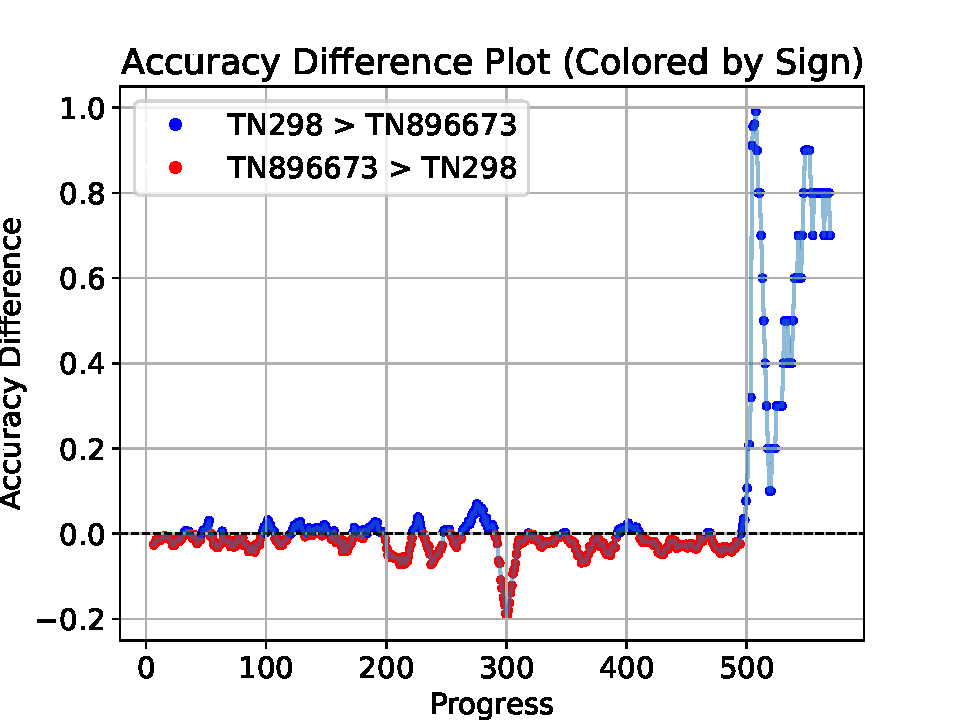
\includegraphics[width=\linewidth]{pdf/compare/merged_NT5_OI1200_compare/acc_diff_plot.pdf}
    \caption{正確度の差分}
    \label{fig:nt5_exp1_acc_diff}
\end{subfigure}
\caption{5タプルネットワーク(EXP1)の評価結果}
\label{fig:nt5_exp1_results}
\end{figure}
    

\begin{figure}[t]
\centering
\begin{subfigure}[b]{0.49\linewidth}
    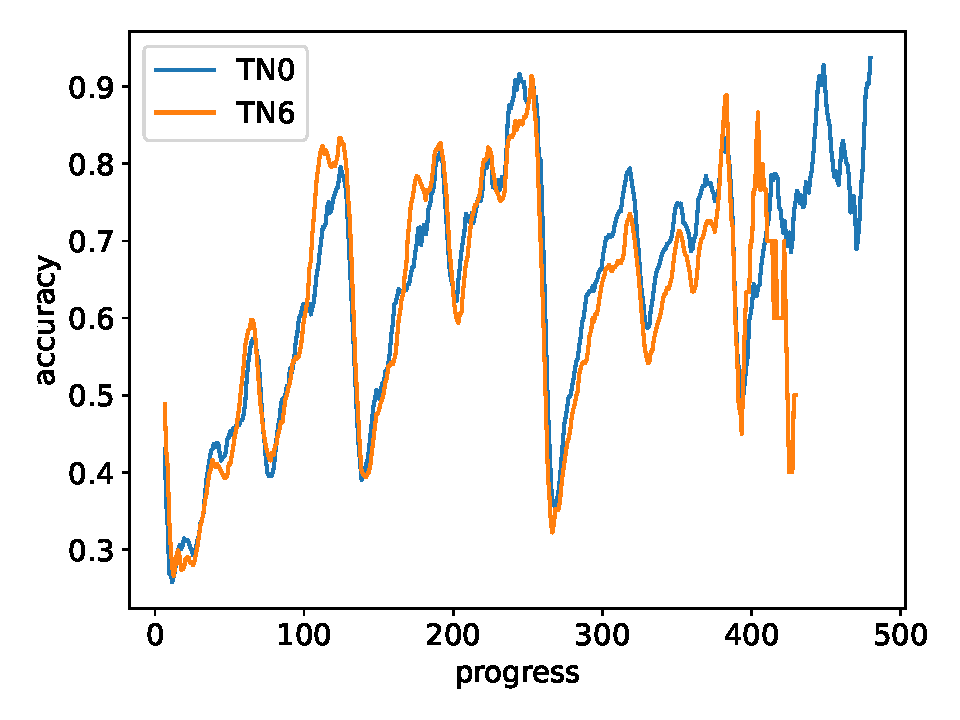
\includegraphics[width=\linewidth]{pdf/compare/merged_NT8_OI1200_compare/accuracy.pdf}
    \caption{正確度}
    \label{fig:nt8_exp1_accuracy}
\end{subfigure}
\begin{subfigure}[b]{0.49\linewidth}
    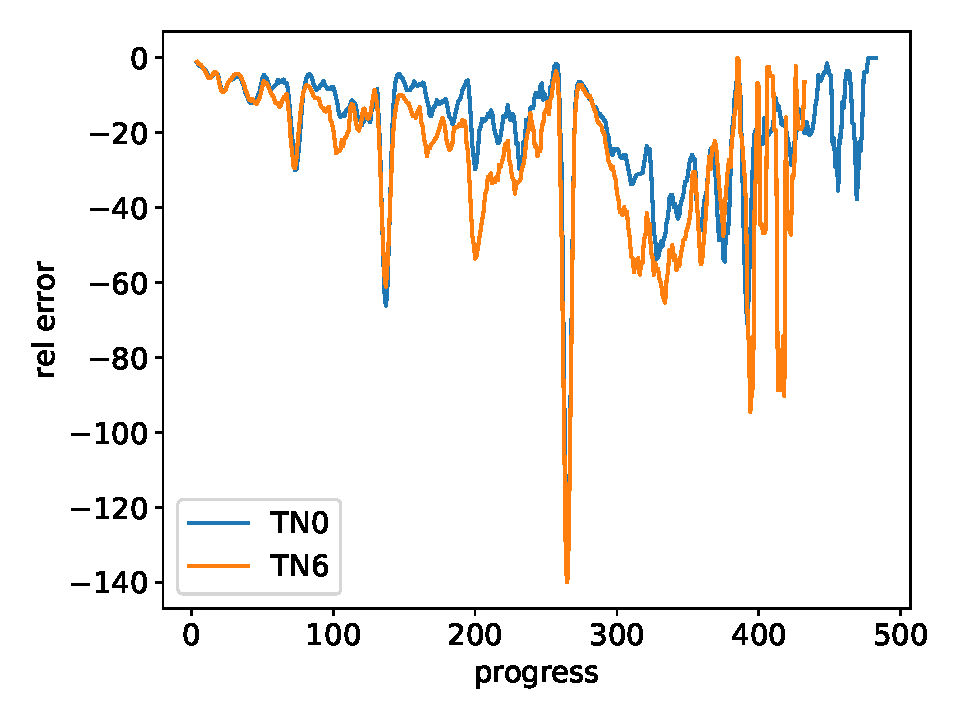
\includegraphics[width=\linewidth]{pdf/compare/merged_NT8_OI1200_compare/error_abs.pdf}
    \caption{絶対誤差}
    \label{fig:nt8_exp1_error_abs}
\end{subfigure}
% \begin{subfigure}[b]{0.49\linewidth}
%     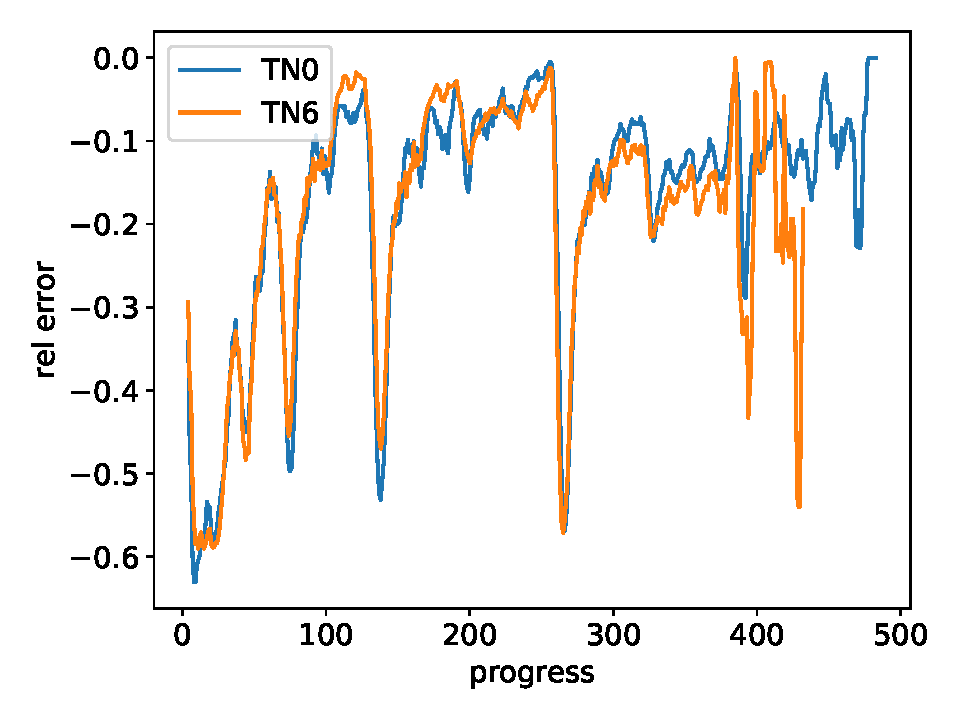
\includegraphics[width=\linewidth]{pdf/compare/merged_NT8_OI1200_compare/error_rel.pdf}
%     \caption{相対誤差}
%     \label{fig:nt8_exp1_error_rel}
% \end{subfigure}
\begin{subfigure}[b]{0.49\linewidth}
    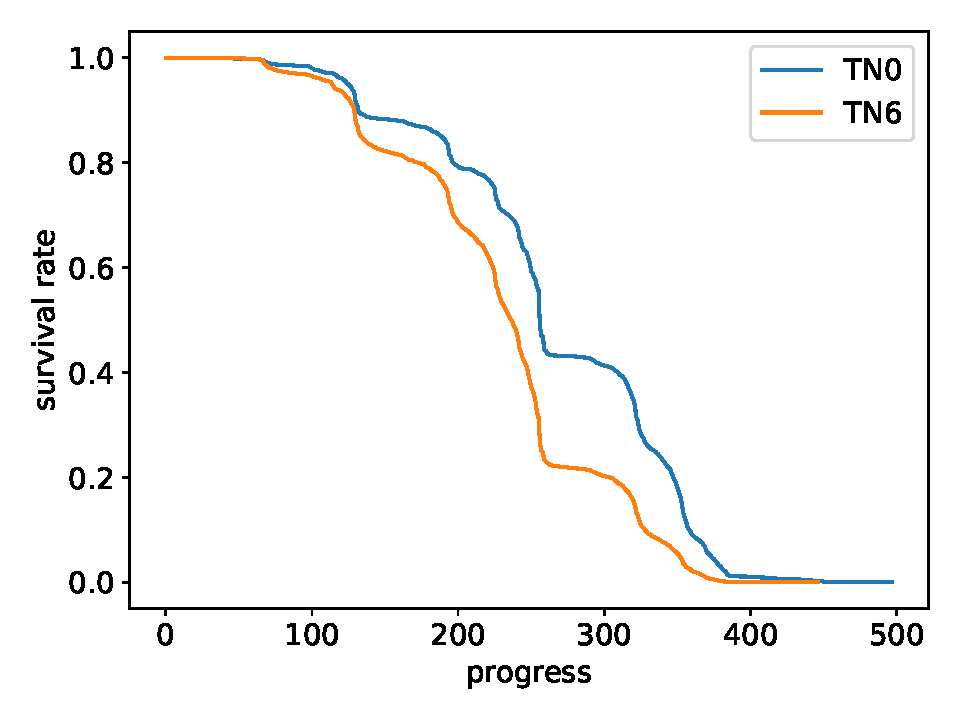
\includegraphics[width=\linewidth]{pdf/compare/merged_NT8_OI1200_compare/survival.pdf}
    \caption{生存率}
    \label{fig:nt8_exp1_survival}
\end{subfigure}
\begin{subfigure}[b]{0.49\linewidth}
    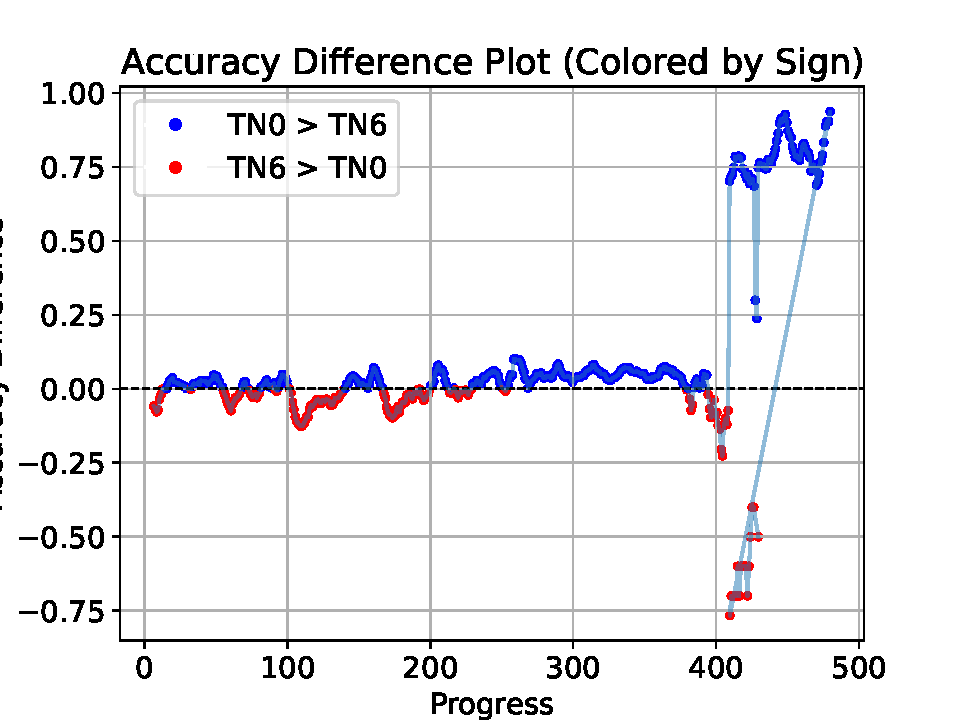
\includegraphics[width=\linewidth]{pdf/compare/merged_NT8_OI1200_compare/acc_diff_plot.pdf}
    \caption{正確度の差分}
    \label{fig:nt8_exp1_acc_diff}
\end{subfigure}
\caption{8タプルネットワーク(EXP1)の評価結果}
\label{fig:nt8_exp1_results}
\end{figure}
    

\begin{figure}[t]
\centering
\begin{subfigure}[b]{0.49\linewidth}
    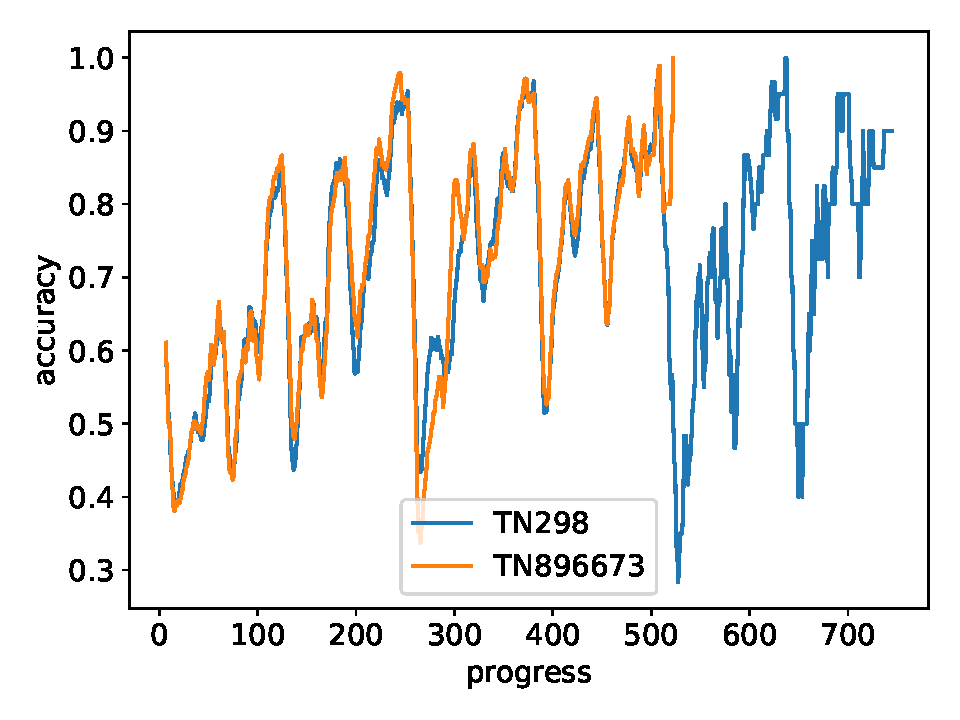
\includegraphics[width=\linewidth]{pdf/compare/merged_EXP_5_NT5_OI1200_compare/accuracy.pdf}
    \caption{正確度}
    \label{fig:nt5_exp5_accuracy}
\end{subfigure}
\begin{subfigure}[b]{0.49\linewidth}
    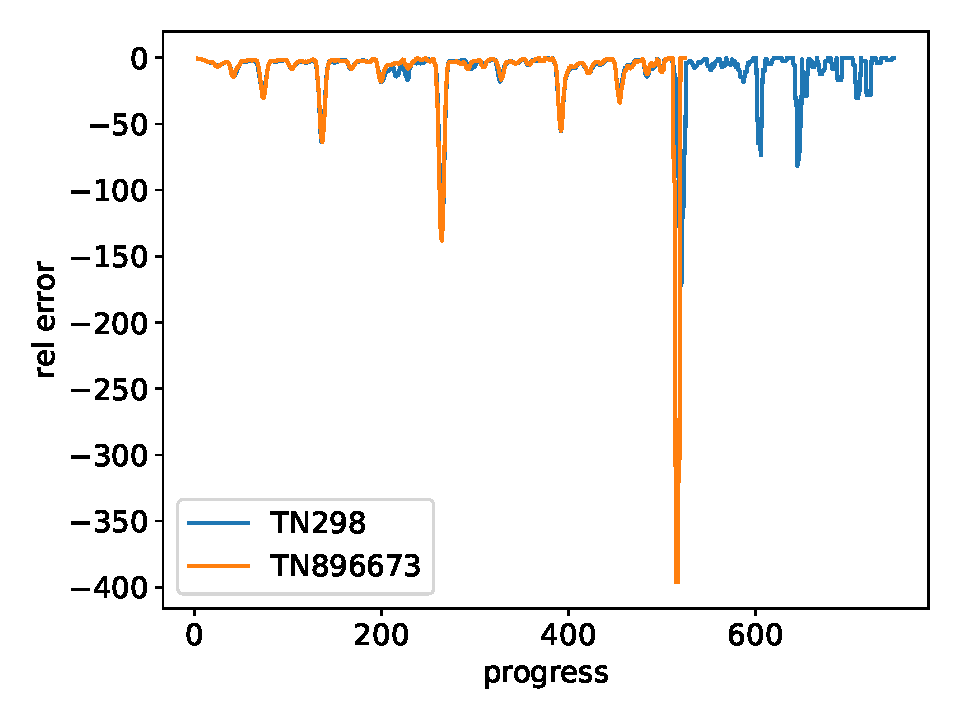
\includegraphics[width=\linewidth]{pdf/compare/merged_EXP_5_NT5_OI1200_compare/error_abs.pdf}
    \caption{絶対誤差}
    \label{fig:nt5_exp5_error_abs}
\end{subfigure}
% \begin{subfigure}[b]{0.49\linewidth}
%     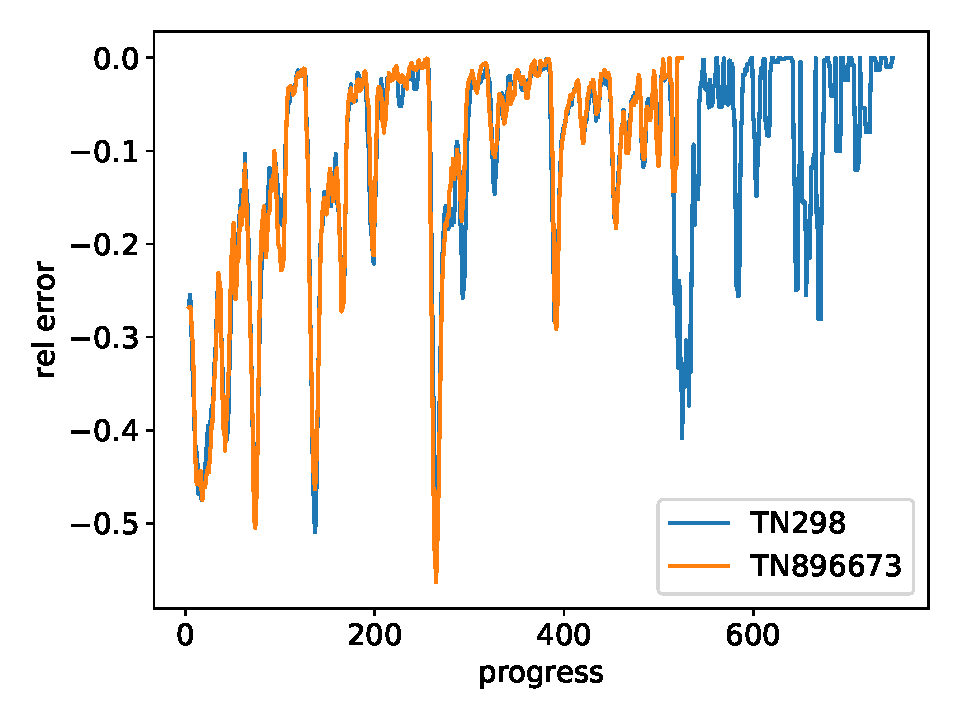
\includegraphics[width=\linewidth]{pdf/compare/merged_EXP_5_NT5_OI1200_compare/error_rel.pdf}
%     \caption{相対誤差}
%     \label{fig:nt5_exp5_error_rel}
% \end{subfigure}
\begin{subfigure}[b]{0.49\linewidth}
    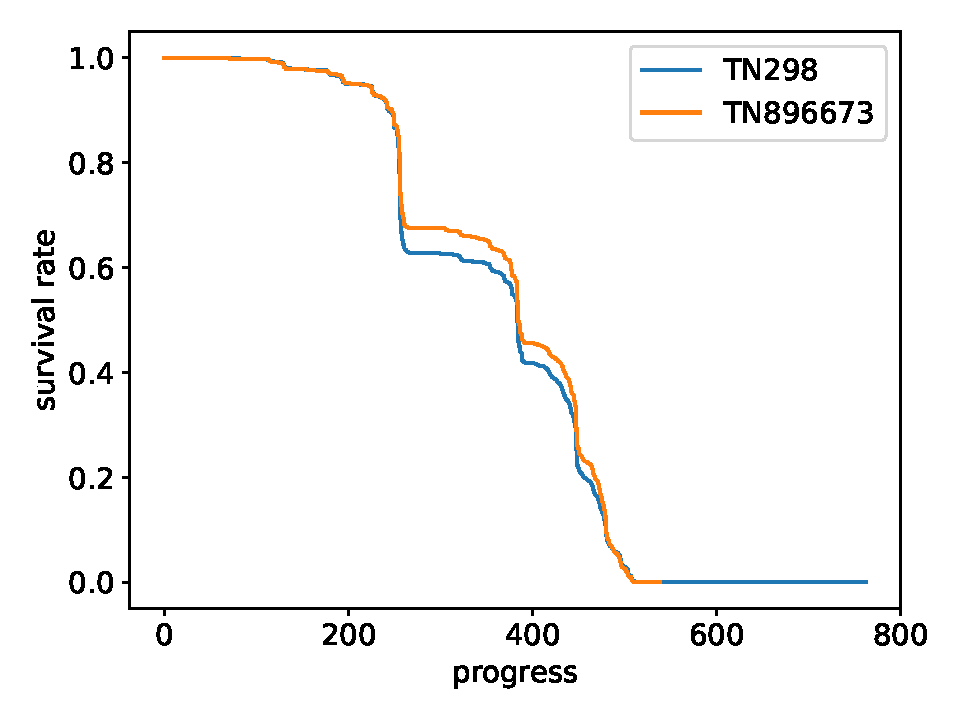
\includegraphics[width=\linewidth]{pdf/compare/merged_EXP_5_NT5_OI1200_compare/survival.pdf}
    \caption{生存率}
    \label{fig:nt5_exp5_survival}
\end{subfigure}
\begin{subfigure}[b]{0.49\linewidth}
    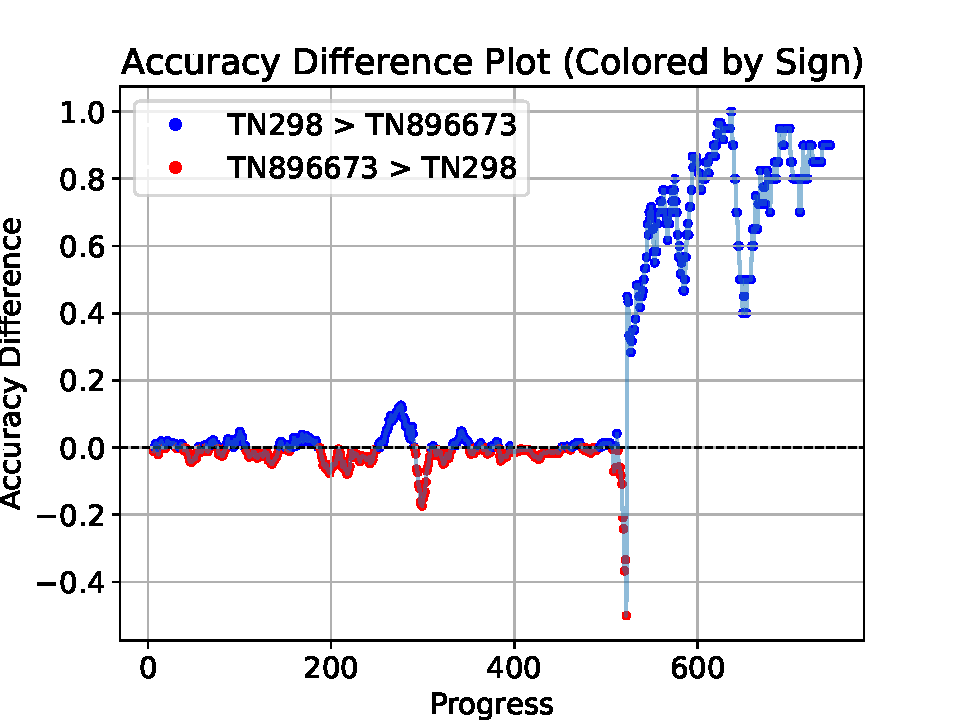
\includegraphics[width=\linewidth]{pdf/compare/merged_EXP_5_NT5_OI1200_compare/acc_diff_plot.pdf}
    \caption{正確度の差分}
    \label{fig:nt5_exp5_acc_diff}
\end{subfigure}
\caption{5タプルネットワーク(EXP5)の評価結果}
\label{fig:nt5_exp5_results}
\end{figure}
    

\begin{figure}[t]
\centering
\begin{subfigure}[b]{0.49\linewidth}
    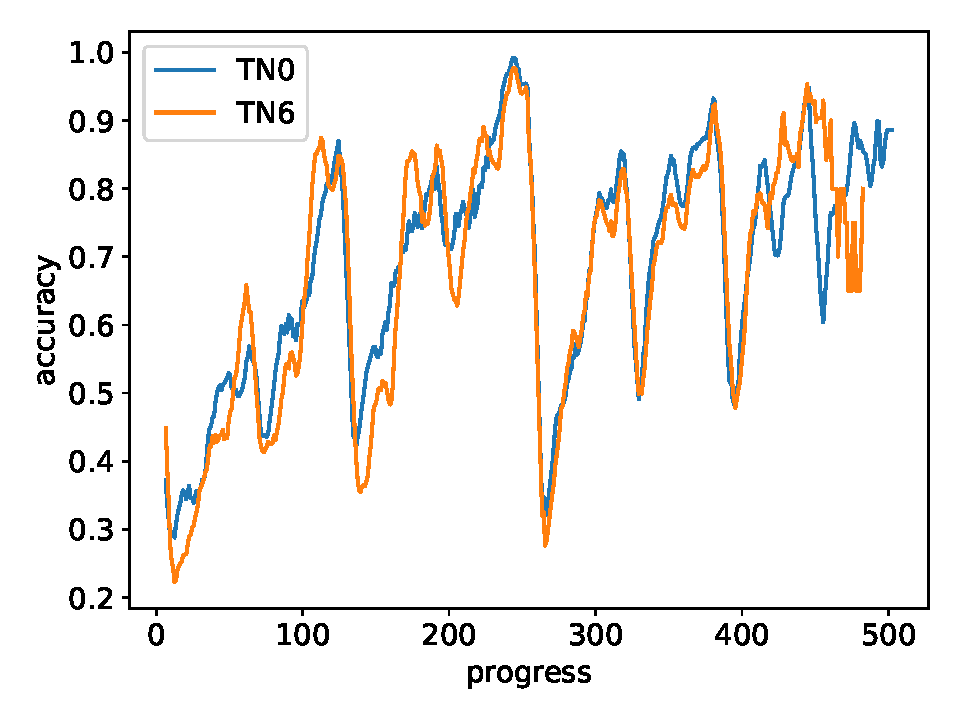
\includegraphics[width=\linewidth]{pdf/compare/merged_EXP_5_NT8_OI1200_compare/accuracy.pdf}
    \caption{正確度}
    \label{fig:nt8_exp5_accuracy}
\end{subfigure}
\begin{subfigure}[b]{0.49\linewidth}
    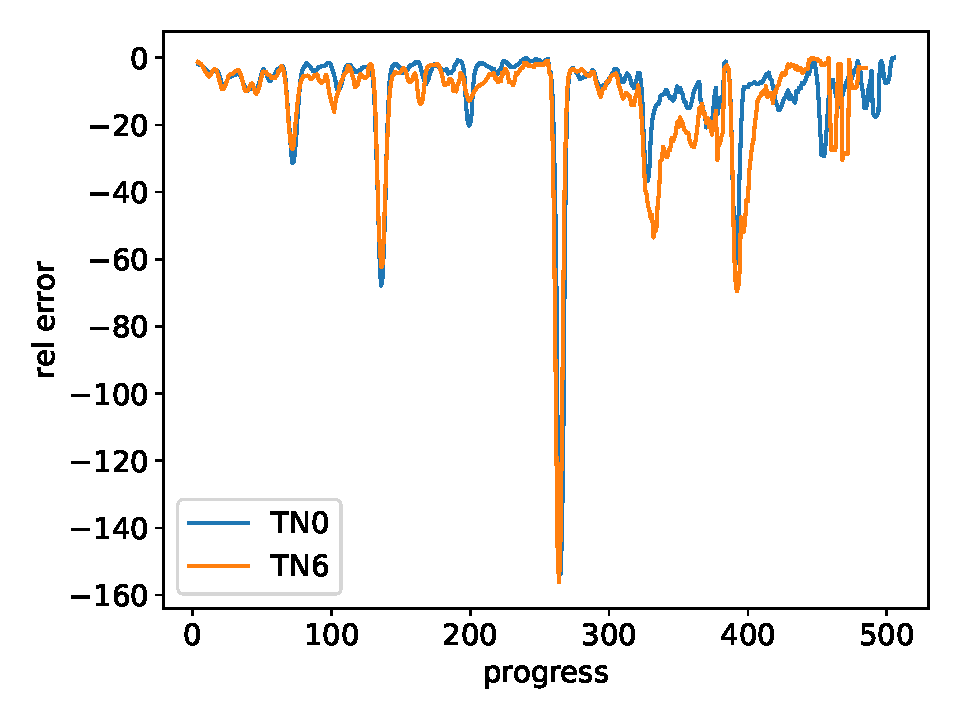
\includegraphics[width=\linewidth]{pdf/compare/merged_EXP_5_NT8_OI1200_compare/error_abs.pdf}
    \caption{絶対誤差}
    \label{fig:nt8_exp5_error_abs}
\end{subfigure}
% \begin{subfigure}[b]{0.49\linewidth}
%     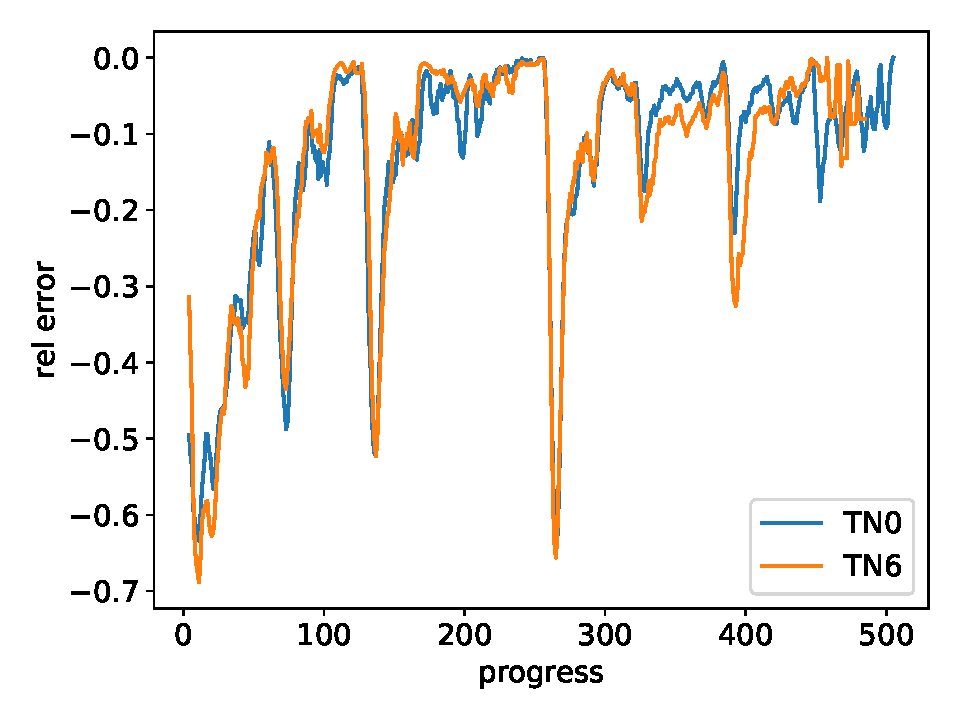
\includegraphics[width=\linewidth]{pdf/compare/merged_EXP_5_NT8_OI1200_compare/error_rel.pdf}
%     \caption{相対誤差}
%     \label{fig:nt8_exp5_error_rel}
% \end{subfigure}
\begin{subfigure}[b]{0.49\linewidth}
    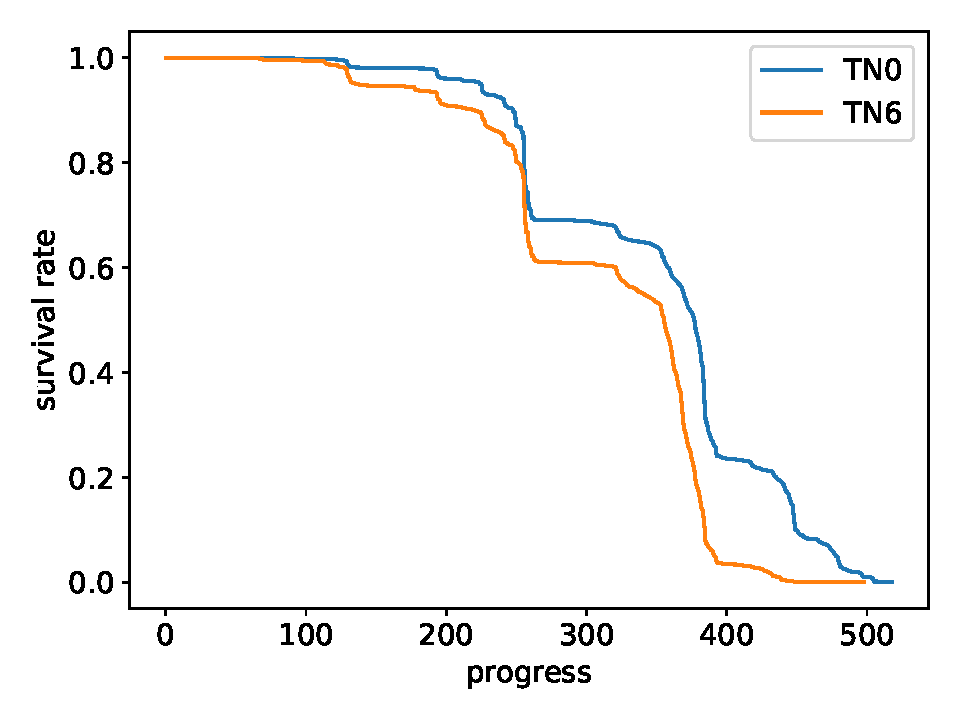
\includegraphics[width=\linewidth]{pdf/compare/merged_EXP_5_NT8_OI1200_compare/survival.pdf}
    \caption{生存率}
    \label{fig:nt8_exp5_survival}
\end{subfigure}
\begin{subfigure}[b]{0.49\linewidth}
    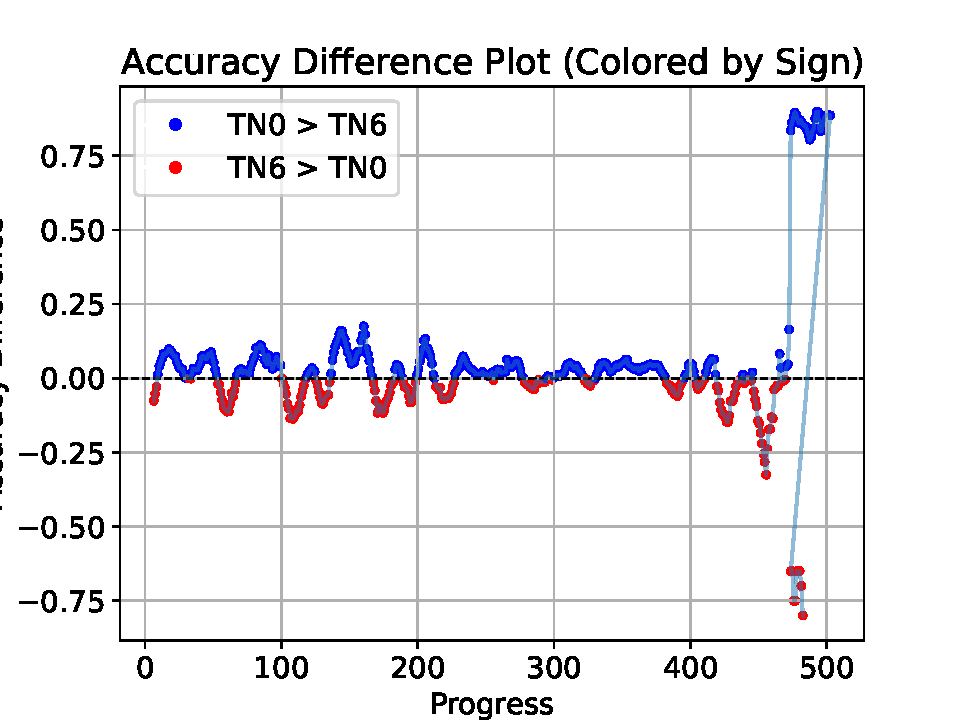
\includegraphics[width=\linewidth]{pdf/compare/merged_EXP_5_NT8_OI1200_compare/acc_diff_plot.pdf}
    \caption{正確度の差分}
    \label{fig:nt8_exp5_acc_diff}
\end{subfigure}
\caption{8タプルネットワーク(EXP5)の評価結果}
\label{fig:nt8_exp5_results}
\end{figure}

これらの結果からTNが変わってもプレイヤの動きにはあまり変化がなく
学習が正確な判断ができる場合とそうではない場合があるが、
良いタプルの組み合わせを選ぶことで、何もないような盤面でのミスが減ることが分かった。
またタプルの数を増やすことは6タプル以上の場合有効ではないことも確認できた。